\documentclass[a4paper, 12pt]{extarticle}

\usepackage[a4paper, total={6.5in, 9in}]{geometry}

\usepackage{tkz-euclide}

\usepackage{amssymb}
\usepackage{amsfonts}
\usepackage{enumitem}
\usepackage{stmaryrd}
\usepackage{amsmath}
\usepackage{easybmat}
\usepackage{tikz}

%-------------------------------commands definitionen-------------------------------
% Für methoden die eine fallunterscheidung haben aufrufen mit: 
% \twopartdef 	{x} {x \geq 0} 
%				{-x} {x < 0} 
%(bsp. Betrag)
\newcommand{\twopartdef}[4] {
	\left\{
		\begin{array}{ll}
			#1 & #2 \\
			#3 & #4
		\end{array}
	\right.
}
% Für methoden mit 3 fällen zwischen denen entschieden werden muss
\newcommand{\threepartdef}[6] {
	\left\{
		\begin{array}{lll}
			#1 &  #2 \\
			#3 &  #4 \\
			#5 &  #6
		\end{array}
	\right.
}
% Am besten immer die befehle Einrücken, damit man erkennt welche Matrix dargestellt wird.
% Z.B.: \twoXtwo{1}{2}
%				{3}{4}
\newcommand{\twoXtwo}[4] {
	\left( 
	\begin{matrix}
		#1 & #2 \\
		#3 & #4
	\end{matrix} 
	\right)
}
\newcommand{\twoXthree}[6] {
	\left( 
	\begin{matrix}
		#1 & #2 & #3\\
		#4 & #5 & #6
	\end{matrix} 
	\right)
}
\newcommand{\threeXtwo}[6] {
	\left( 
	\begin{matrix}
		#1 & #2 \\
		#3 & #4 \\
		#5 & #6
	\end{matrix} 
	\right)
}
\newcommand{\threeXthreeNoBracket}[9]{
	\begin{matrix}
		#1 & #2 & #3\\
		#4 & #5 & #6\\
		#7 & #8 & #9
	\end{matrix}
}
\newcommand{\threeXthree}[9] {
	\left( 
	\begin{matrix}
		#1 & #2 & #3\\
		#4 & #5 & #6\\
		#7 & #8 & #9
	\end{matrix}
	\right)
}
%Vektoren, sind quasi nx1 matrizen
\newcommand{\vecTwo}[2] {
	\left( 
	\begin{matrix}
		#1\\
		#2
	\end{matrix} 
	\right)
}
\newcommand{\vecThree}[3] {
	\left( 
	\begin{matrix}
		#1\\
		#2\\
		#3
	\end{matrix} 
	\right)
}
% Zur besseren Lesbarkeit der Norm-Schreibweise
\newcommand{\norm}[1]{
	\parallel #1 \parallel
}
% Befehl für das Skalarprodukt
\newcommand{\skalar}[2] {
	\langle #1, #2\rangle
}

% Wortersetzung für Skalarprodukt mit cdots drinnen
\newcommand{\genskalar}{
	\skalar{\cdot }{\cdot }
}
% Befehl für skalarprodukt mit 2 mal dem Gleichen Komponenten
\newcommand{\eskalar}[1]{
	\skalar{#1}{#1}
}

% $\Leftrightarrow$ wird zu \gdw
\newcommand{\gdw}{\Leftrightarrow}

% Abkürzung von \textnormal
\newcommand{\tn}[1]{\textnormal {#1}}

% Command, um Text leicht transparent zu machen (für Notizen o.Ä.)
\newcommand{\transp}[2][50]{\color{black!#1}#2}
%-----------------------------ende commands definitionen-----------------------------

\begin{document}

\title{Lineare Algebra II - Mitschrift}
\author{Sebastian Pretzsch, Finn Ribbeck, Jonas Heitz}
\maketitle
%------------------------------------Vorlesung 1------------------------------------
\section{Relationen}
Relationen beschreiben Beziehungen zwischen Elementen von Mengen. \\
Wdh. $X{\times}Y := \{(x,y) | x \in X, y \in Y\}$ \\
Menge der (geordneten) Paare, "kartesisches Produkt".

\subsection*{Definition 1.1.}
Seien X,Y Mengen. Eine \textbf{Relation} zwischen X und Y ist eine Teilmenge $R \subseteq X{\times}Y$. \\
\underline{Notation}: für $(x,y)\in R$ auch $xRy$. \\
Falls $X=Y$ sage auch Relation "auf X".

\subsection*{Beispiel}
$X$ Punktmenge, $Y$ Geradenmenge
$$xRy :\Leftrightarrow \tn{Punkt x liegt auf Gerade y}$$

\subsection*{Bemerkung}
Eine Abbildung (Funktion) $f:X{\to}Y$ weist zu jedem $x\in X$ genau ein $
y\in Y$ zu. \\
Wir werden diese fortan als spezielle Relation
$$R_f = \{(x, f(x)) | x\in X\} \subseteq X{\times}Y$$
auffassen. Wir betrachten insbesondere Relation auf X.

\subsection*{Definition 1.2.}
Sei X eine Menge. Eine Relation $R \subseteq X{\times}X$ ist
\begin{enumerate}[label=(\alph*)]
\item \textbf{reflexiv} falls $xRx \hspace*{2mm}\forall x\in X$,
\item \textbf{symmetrisch} falls $xRy \Rightarrow yRx \hspace*{2mm}\forall x,y\in X$ (denn auch "$\Leftarrow$" gilt),
\item \textbf{anti-symmetrisch} falls $xRy \land yRx \Rightarrow x=y$,
\item \textbf{transitiv} falls $xRy \land yRz \Rightarrow xRz$.
\end{enumerate}

\subsection*{Beispiel} 
Sei $X = \mathbb R$.
\begin{enumerate}[label=(\alph*)]
\item $ R:=\{(x,x) | x\in X\}$ (d.h. $xRy \Rightarrow x=y$) erfüllt a), b), c), d).
\item $ xRy :\Leftrightarrow |x|=|y|$ erfüllt a), b), d) (nicht c), da $|1|=|-1|$)
\item $ xRy :\Leftrightarrow x\leq y$ erfüllt a), c), d) (nicht b), da $2\leq 3$ aber $2 \neq 3$
\end{enumerate}
Nun definieren wir die wichtigsten Arten von Relationen.

\subsection*{Definition 1.3.}
Eine Relation R auf X heißt
\begin{enumerate}[label=(\arabic*)]
\item \textbf{Äquivalenzrelation} falls sie reflexiv, symmetrisch und transitiv ist (typische Notation "$\sim$"),
\item \textbf{Ordnungsrelation} falls sie reflexiv, anti-symmetrisch und transitiv ist (Notation "$\leq$").
\end{enumerate}
Im Fall 2. heißt R auch \textbf{(partielle) Ordnung}, und falls 
$$ xRy \lor yRx \hspace*{2mm} \forall x,y \in X$$
zusätzlich gilt \textbf{totale/ lineare Ordnung}.\\
\textbf{Äquivalenzrelationen} auf X entsprechen genau den Zerlegungen von X.
Zwei Mengen A, B heißen \textbf{disjunkt} falls $A \cap B = \emptyset$.

\subsection*{Beispiel}
Kleiner Ausblick:
\begin{enumerate}[label=(\alph*)]
\item Zwei Matrizen $A,B \in \tn{Mat}_{n{\times}m}(K)$ heißen \textbf{ähnlich} falls $S \in \tn{GL}_n(K)$ existiert mit \\$B=S^{-1}{\cdot}A{\cdot}S$.
\item Sei M Menge und $X:=\mathcal P(M)$ Potenzmenge von M\\
 Zu $A,B \in X$ definiere $A\leq B :\Leftrightarrow A\subseteq B$ eine Ordnungsrelation.
\end{enumerate}

%------------------------------------Vorlesung 2------------------------------------
\subsection*{Definition 1.4.}
Sei X Menge. Eine \textbf{Zerlegung} von X ist eine Menge $\mathcal{C}$ von paarweise disjunkten nicht-leeren Mengen $A \subseteq X$ mit $\bigcup_{A \in \mathcal{C}} A = X$.

\subsection*{Beispiel}
Eine Zerlegung von $\{ a, b, c\}$ ist $\{\{ a\}, \{ b, c\}\}$.

\subsection*{Lemma 1.5.}
Sei $\sim$ Äquivalenzrelation auf X und zu $x \in X$ sei $[x] := \{y \in X | x \sim y\} \subseteq X$ ("Klasse" von X).\newline
Dann ist $\mathcal{C} := \{[x] | x \in X\}$ eine Zerlegung von X.\newline
Ferner gilt $x \sim y \Leftrightarrow [x] =  [y]$. (*)\newline
\subsubsection*{Beweis (*)}
"$\Leftarrow$": $y \in [y] = [x] \Rightarrow x \sim y$.\newline
"$\Rightarrow$": Gelte $x \sim y$. Zeige [x] = [y].
\begin{itemize}
\item[--] "$\subseteq$": $z \in [x] \Rightarrow x \sim z \Rightarrow y \sim z \Rightarrow z \in [y]$
\item[--] "$\supseteq$": $z \in [y] \Rightarrow y \sim z \Rightarrow x \sim z \Rightarrow z \in [x]$\newline
\end{itemize}
Zeige $\mathcal{C}$ Zerlegung.\newline
Angenommen $[x] \cap [y] \neq \emptyset \Rightarrow \exists z \in X: z \in [x] \cap [y] \Rightarrow \exists z \in X: x \sim z \sim y \Rightarrow x \sim y \Rightarrow [x] = [y].$\newline Also sind die Klassen paarweise disjunkt (und nicht-leer, da $\forall x \in X: x \in [x]$).\newline Wegen $\forall x \in X: x \in [x]$ gilt außerdem $\bigcup_{x \in X} [x] = X$.

\begin{flushleft}
$\square$\\
\end{flushleft}

\subsection*{Beispiel}
\begin{enumerate}[label=(\alph*)]
\item $X = \mathbb{R}, x \sim y :\Leftrightarrow |x| = |y|$.
Zerlegung von $\mathbb{R}$ ist $\{\{0\}\} \cup \{\{a, -a\} | a \in \mathbb{R}_{>0}\}$.
\item $X = \mathbb{Z}, n \in \mathbb{N}_{>0}$, betrachte $x \sim y :\Leftrightarrow n | x - y \Leftrightarrow y = x + k \cdot n$ für ein $k \in \mathbb{Z}$.
Zerlegung von $\mathbb{Z}$ ist $\{0 + n\mathbb{Z},\ldots, (n - 1) + n\mathbb{Z}\}$ (n Klassen).
\end{enumerate}

\subsection*{Definition 1.6.}
Die Zerlegung von X bezüglich der Relation $\sim$ heißt Zerlegung in \textbf{Äquivalenzklassen}. Notation für $\mathcal{C}$ auch X/$\sim$, "X modulo $\sim$".
\subsubsection*{Bemerkung}
Umgekehrt definiert jede Zerlegung $\mathcal{C}$ von X Äquivalenzrelation $\sim_\mathcal{C} := \bigcup_{A \in \mathcal{C}} A \times A \subseteq X \times X$ (Übung) und die Konstruktionen sind zueinander invers.

\subsection*{Beispiel}
Es gibt fünf Zerlegungen von $X = \{a, b, c\}$. Die Kreuztabellen der zugehörigen Äquivalenzrelationen lauten:
\begin{tabbing}
\=
\begin{tabular}[h]{cccc}
 & a & b & c \\
a & X & & \\
b & & X & \\
c & & & X \\
\end{tabular}
\=
\begin{tabular}[h]{cccc}
 & a & b & c \\
a & X & X & \\
b & X & X & \\
c & & & X \\
\end{tabular}
\=
\begin{tabular}[h]{cccc}
 & a & b & c \\
a & X & & X \\
b & & X & \\
c & X & & X \\
\end{tabular}
\=
\begin{tabular}[h]{cccc}
 & a & b & c \\
a & X & & \\
b & & X & X \\
c & & X & X \\
\end{tabular}
\=
\begin{tabular}[h]{cccc}
 & a & b & c \\
a & X & X & X \\
b & X & X & X \\
c & X & X & X \\
\end{tabular}
\\
\>$\{\{a\}, \{b\}, \{c\}\}$
\>$\{\{a, b\}, \{c\}\}$
\>$\{\{a, c\}, \{b\}\}$
\>$\{\{b, c\}, \{a\}\}$
\>$\{\{a, b, c\}\}$\\
\end{tabbing}
Zusammenhang mit Abbildungen:
\subsubsection*{Bemerkung}
Jede Äquivalenzrelation $\sim$ auf X definiert eine (surjektive) Abbildung\\
$\pi: X \longrightarrow X/\sim, x \longmapsto [x]$.\\
Umgekehrt definiert jede Abbildung $f: X \longrightarrow Y$ eine Äquivalenzrelation auf X durch\\ $x \sim x' :\Leftrightarrow f(x) = f(x')$.

\subsection*{Wichtige Begriffe zu Ordnung}
Sei (X, $\leq$) geordnete Menge. Darstellung (im endlichen Fall) als Diagramm mit Verbindungen \begin{tabular}{c}
b \cr $\mid$ \cr a
\end{tabular} falls $a < b$ und es existiert kein $c$ mit $a < c < b$ "Nachbarschaftsrelation".

\subsection*{Beispiel}
siehe Vorlesung (15.04.21 / 56:20)

\subsection*{Definition 1.7.}
Sei (X, $\leq$) geordnete Menge. Elemente $a, b \in X$ heißen \textbf{vergleichbar} falls $a \leq b \lor b \leq a$.\\
Teilmenge $Y \subseteq X$ heißt \textbf{Kette} falls alle $a, b \in Y$ vergleichbar (d.h. X ist Kette gdw. X total geordnet).
\begin{tabbing}
Ein Element $a \in X$ heißt \= \textbf{maximal} falls $\forall x \in X: x \geq a \Rightarrow x = a$,\\ \>\textbf{größtes Element} falls $\forall x \in X: x \leq a$.\\ \>\textbf{obere Schranke} von $Y \subseteq X$ falls $\forall y \in Y: y \leq a$.\\
Dual dazu: minimal, kleinstes Element, untere Schranke\\
\end{tabbing}

\subsection*{Beispiel}
$\mathcal{P}(M)\backslash\{\emptyset\}$ hat als minimale Elemente $\{m\}$ wobei $m \in M$.\\
z.B.: $M:=\{a, b\} \rightarrow \mathcal{P}(M)\backslash\{\emptyset\} = \{\{a\}, \{b\}, \{a, b\}\}$ hat minimale Elemente $\{a\}$ und $\{b\}$.
%----------------------------------Vorlesung 3----------------------------------
\section{Unendliche Mengen und Lemma von Zorn}
Notation: Zu $n\in\mathbb{N}$ sei $[n]:= \{1,2...,n\} $.

\subsection*{Definition 2.1.}
Eine Menge $X$ heißt endlich, falls $\exists n \in \mathbb{N}$ und Bijektion $\phi: X \rightarrow [n]$; in diesem Fall heißt $n$ die Kardinalität $|X|$ oder $\#X$ von $X$.
Ansonsten heißt $X$ unendlich. 
\subsubsection*{Bemerkung (Taubenschlagprinzip)}
Ist $n>m$, so ist jede Abbildung $f: [n] \rightarrow [m]$ nicht injektiv, das heißt $\exists x\neq x'$ ("Tauben") mit $f(x) = f(x')$. \\
Es folgt: Ist $\phi : [n] \rightarrow [m]$ bijektiv, so gilt $n=m$. Somit ist die Kardinalität eindeutig.

\subsection*{Beispiel}
Menge $X = \{a,b,c,d\}$ ist endlich mit Kardinalität 4, \\
$\#X =  4$ mögliche Bijektion: 
\begin{tabular}{cccc}
$a \rightarrow 1$ & $c \rightarrow 3$ \\
$b \rightarrow 2$ & $d \rightarrow 4$ \\
\end{tabular}
\\
\\
Der Umgang mit unendlichen Mengen erfordert oft "Auswahlaxiom".

\subsection*{Bemerkung}
Abbildung $f: X \rightarrow Y$ ist injektiv $\Leftrightarrow \exists g: Y \rightarrow X : g \circ f = id_x$ ($X \neq \emptyset $).
\subsubsection*{Beweis}
$"\Leftarrow"$ \\
$x,x' \in X :$
$f(x) = f(x') \Rightarrow  x = g(f(x)) = g(f(x'))$ nach Voraussetzung.\\
Also ist f injektiv. \\ 
\\
$"\Rightarrow"$\\
Sei $Y_0 := im f$ und betrachte $f_0 : X \rightarrow Y_0$, $f_0(x) := f(x)$ ist bijektiv \\
 $\Rightarrow \exists g_0 := f_0^{-1}: Y_0 \rightarrow X$,\\
setze fort zu $g: Y \rightarrow X$,\\
das heißt $g(y) := g_0(y)$ für $y\in Y_0$, sonst beliebig.\\
$\Rightarrow g(f(x)) = x \forall  x \in X (f(x) \in Y_0)$.\\
\begin{flushright}
$\square$\\
\end{flushright}
Gilt $f \circ g = id_y$, so ist $f$ surjektiv: zu $y\in Y \exists x:= g(y)$ mit $f(x) = y$.\\
Umgekehrt gilt:
\subsection*{Axiom 2.2. (Auswahlaxiom)}
Jede surjektive Abbildung $f: X \rightarrow Y$ besitzt eine Rechtsinverse, das heißt \\
$g: Y \rightarrow X$ mit $f \circ g = id_y$.\\
Äquivalente Formulierung:\\
Sei $(A_i)_{i \in I}$ Familie von nicht-leeren Teilmengen von X.\\
Dann existiert $(a_i)_{i \in I}$ mit $a_i \in A_i \forall i \in I$.\\
(Kurz: $X_{i \in I} A_i \neq \emptyset $)
\subsubsection*{"Beweis"}
Jedes $y \in Y$ hat ein Urbild $x \in X$ mit $f(x) = y$.\\
Definiere also $g: Y \rightarrow X$ durch $Y \rightarrow X$ mit $f(x) = y$.\\
Dass eine solche Auswahl stets existiert, besagt das Axiom.

\subsection*{Definition 2.3.}
Zwei Mengen $X,Y$ heißen gleichmächtig, falls eine Bijektion $\phi: X \rightarrow Y$ existiert; $X$ hat Mächtigkeit $Y$.(Dies erfüllt Eigenschaften einer Äquivalenzrelation)\\
Eine Menge $X \neq \emptyset$ heißt abzählbar, falls Surjektion $\mathbb{N} \rightarrow X$ existiert. ($\emptyset$ sei abzählbar; $f: \mathbb{N} \rightarrow X$ surjektiv $\Rightarrow X = \{f(0), f(1), ...\}$), das heißt (Auswahlaxiom) falls  Injektion $X \rightarrow \mathbb{N}$ besteht.\\
Andernfalls heißt $X$ überabzählbar.

\subsection*{Bemerkung}
\begin{enumerate}[label=(\arabic*)]
\item abzählbar unendlich  $\Leftrightarrow$ Mächtigkeit $\mathbb{N}$
\item existiert $f: X \rightarrow \mathbb{N}$ mit endlichen Urbildern $f^{-1}(\{n\}) \forall n\in \mathbb{N}$, so ist $X$ abzählbar.
\end{enumerate}

\subsection*{Satz 2.4.}
$\mathbb{Q}$ ist abzählbar.
\subsubsection*{Beweis (1. Cantorscher Diagonalbeweis)}
siehe Vorlesung.

\subsection*{Satz 2.5.}
\begin{enumerate}[label=(\alph*)]
\item $\mathbb{R}$ ist überabzählbar.
\item Für jede Menge $X$ ist $P(X)$ nicht gleichmächtig zu $X$.
\end{enumerate}
\subsubsection*{Beweis (2. Cantorscher Diagonalbeweis)}
siehe Vorlesung.
%------------------------------------Vorlesung 4------------------------------------
\subsection*{Satz 2.6. (Lemma von Zorn)}
Sei $(X, \leq)$ geordnete Menge sodass jede Kette in $Y \subseteq X$ eine obere Schranke hat. Dann hat $X$ ein maximales Element.\\
\subsubsection*{Diskussion:}
\begin{enumerate}[label=(\arabic*)]
\item Nicht interessant (trivial) für $X$ endlich, oder für $(X,\leq )$ total geordnet: betrachte Kette $Y=X$.
\item Anwendungsfall oft $X\subseteq \mathcal P(M)$. Kette $Y\subseteq X$ hat obere Schranke z.B. 
falls $\bigcup_{A\in Y}A\in X$ gilt.
\item Beweis ist technisch anspruchsvoller (Mengenlehre) und benutzt Auswahlaxiom; umgekehrt kann Auswahlaxiom aus Zorn folgern (vgl. Halmos).
\end{enumerate}
Nun zu Basen für beliebige Vektorräume. \\
In Lineare Algebra I haben wir gesehen, dass jeder endlich erzeugte K-Vektorraum V eine (endliche) Basis $S\subseteq V$ hat; \\
Dann gilt $V\cong K^n$, $n:=\tn{dim}_KV$.\\
\underline{Erinnerung:} Eine Teilmenge $S\subseteq V$ heißt Erzeugendensystem falls 
$$span \hspace*{1mm} S := \{\sum_{i=1}^n
\lambda_i v_i | \lambda_i \in K, v_i \in S, n \in \mathbb N\} = V \tn{ gilt.}$$
Und $S\subseteq V$ heißt linear unabhängig falls $\sum_{i=1}^n \lambda_i v_i = 0$ mit $v_i\in S$ verschieden stets $\lambda_i = 0$, $\forall i$ impliziert.
\subsection*{Proposition 2.7.}
Zu I Menge sei $K^{(I)} := \{f:I\rightarrow K | f(i) \neq 0$ nur für endliche viele $i\in I\}$. \\
Dann ist $K^{(I)}$ ein K-Vektorraum mit Basis $\{e_i|i\in I\}$, wobei $e_i(j):= \twopartdef { 1 } {\tn{falls } j=i} {0} {\tn{sonst}}$. \\
Umgekehrt ist jeder K-Vektorraum mit Basis isomorph zu einem $K^{(I)}$.
\subsubsection*{Beweis:}
\begin{itemize}
\item[--] "K-Vektorraum": $K^{(I)}$ ist Untervektorraum von $K^I := \{f:I\rightarrow K\}$.
\item[--] "Erzeugendensystem": sei $f\in K^{(I)}$ und sei $I_0 := \{i_1,...,i_n\} \subseteq I$ mit $f(i) = 0$ $\forall i \notin I_0;$ setze $\lambda_k := f(i_k)$, $k=1,...n$ 
$$ \Rightarrow f = \sum_{k=1}^n \lambda_k e_{i_k}\tn{, denn }\lambda_j = f(i_j) = \sum_{k=1}^n \lambda_k e_{i_k}(i_j) = \lambda_j, \hspace*{1mm} \forall j = 1,...,n$$
\item[--] "linear unabhängig": angenommen $\sum \lambda_k e_{i_k} = 0 \Rightarrow \lambda_j = \sum \lambda_k e_{i_k}(i_j) = 0$ $\forall j$
\end{itemize}
Zusatz: Sei V ein K-Vektorraum mit Basis $\{e_i | i \in I\}$, so ist die Linearkombinationsabbildung (vgl. Lin-Alg.I, Bem. 8.3)
$\gamma: K^{(I)} \rightarrow V$, $f\mapsto \sum_{i\in I} f(i)e_i$ ein K-Isomorphismus.
\begin{flushright}
$\square$\\
\end{flushright}
\subsection*{Bemerkung}
$K^{(I)}=K^I \Leftrightarrow$ I endlich. \\
Aber z.B. ist $\mathbb Q^{(\mathbb N)}$ abzählbar und $\mathbb Q^\mathbb N$ überabzählbar (Übung). \\
Basen z.B. für $K^I$?
\subsection*{Satz 2.8.}
Jeder Vektorraum besitzt eine Basis.
\subsubsection*{Beweis (via Lemma von Zorn)}
Sei V ein K-Vektorraum und sei $X \subseteq \mathcal P(V)$ die Menge aller linear unabhängigen Teilmengen $S \subseteq Y$. \\
Sei $Y\subseteq X$ Kette. Behauptung: $T:=\bigcup_{S\in Y} S$ ist linear unabhängig. \\
Gelte $\sum_{i=1}^n \lambda_i v_i = 0$ mit $\lambda_i \in K$ und $v_i \in T$ verschieden. \\
$$\Rightarrow \exists S_i \in Y\tn{ mit }v_i \in S_i\tn{, }\forall i=1,...n$$
$$\Rightarrow_{\tn(S_1,...,S_n \tn{Kette)}} \exists i_0\tn{ mit }S_i \subseteq S_{i_0}\tn{, } \forall i\tn{, somit }v_i \in S_{i_0}$$
$$\Rightarrow_{S_{i_0}\tn{ lin. unabh.}}\tn{ alle }\lambda_i=0$$
$$\Rightarrow_{\tn{Satz 2.6 (Zorn)}}\tn{ es existiert ein maximales Element S in X.}$$
Behauptung dieses S ist auch erzeugend (dann fertig).\\
Angenommen es existiert $v\in V\backslash\tn{span }S$ sei $S':= S\cup \{v\}$. Dann ist S' linear unabhängig.\\
Betrachte $\sum_{i=1}^n\lambda_iv_i=0$ mit $v_i\in S'$ verschieden.
\begin{itemize}
\item falls alle $v_i\in S \Rightarrow$ alle $\lambda_i = 0$
\item sonst $\lambda v = \sum \lambda_j v_j$, wäre $\lambda \neq 0 \Rightarrow v\in \tn{span }S \lightning$\\
$\Rightarrow \lambda = 0 \Rightarrow$ alle $\lambda_j=0$
\end{itemize}
Weil aber $S\subsetneq S'$ Widerspruch zur Maximalität von S.
\begin{flushright}
$\square$\\
\end{flushright}
%----------------------------------Vorlesung 5----------------------------------
\section{Äquivalenz von Matrizen}
\textbf{Wiederholung} (Lin. Alg. I).\\ Seien $V, W$ K-Vektorräume mit Basen $\mathcal{B} = (v_1, \dots, v_n)$ von $V$ und $\mathcal{C} = (w_1, \dots, w_m)$ von $W$. \\
Zu $f: V \longrightarrow W$ linear ist $A = {_\mathcal B}M_\mathcal{C}(f) \in Mat_{m\times n}(K)$ gegeben durch:\\
\begin{tabbing}
	\hspace{15pt}\=\hspace{40pt}\=\hspace{40pt}\= \kill
	\>$V \xrightarrow f$ \>$W$ $\xrightarrow g$ \>$X$\\
	$\Phi{_\mathcal B}$ \>$\uparrow$ \>$\uparrow \Phi_\mathcal{C}$ \>$\uparrow \Phi_\mathcal{D}$\\
	\>$K^n \xrightarrow{f_A}$ \>$K^m$ $\xrightarrow{f_B}$ \>$K^l$\\
\end{tabbing}
d.h. $f_A = \Phi_\mathcal{C}^{-1}\circ f \circ \Phi{_\mathcal B}$. Ist auch $X$ K-Vektorraum mit Basis $\mathcal{D} = (x_1, \dots, x_l)$ und $g: W \longrightarrow X$ linear, so gilt ${_\mathcal B}M_\mathcal{D}(g \circ f) = _\mathcal{C}M_\mathcal{D}(g) \cdot {_\mathcal B}M_\mathcal{C}(f) = B \cdot A$.\\ \\
Wie verändert sich die darstellende Matrix bei einem Basiswechsel?\\
Betrachte Diagramm zu zwei Basen $B$ und $B'$ von $V$\\
\begin{tabbing}
	\hspace{15pt}\=\hspace{40pt}\=\hspace{2cm}\= \kill
	\>$V \xrightarrow{id_V}$ \>$V$\\
	$\Phi{_\mathcal B}$ \>$\uparrow$ \>$\uparrow \Phi_\mathcal{B'}$\\
	\>$K^n \xrightarrow{f_\mathcal{T}}$ \>$K^n$ \>d.h. $f_\mathcal{T} = \Phi_\mathcal{B'}^{-1} \circ \Phi{_\mathcal B}$\\
\end{tabbing}
Die Matrix $\mathcal{T} := {_\mathcal B}M_\mathcal{B'}(id_V) \in \mathcal{G}L_n(K)$ heißt \textbf{Transformationsmatrix}\\
(d.h. $v_j = \sum_{i=1}^{n} t_{ij} v_i'$ mit $\mathcal{B} = (v_1, \dots, v_n), \mathcal{B'} = (v_1', \dots, v_n')$). $\mathcal{T}^{-1} = _\mathcal{B'}M{_\mathcal B}(id_V)$\\

\subsection*{Satz 3.1. (Transformationsformel)}
Gegeben seien K-Vektorräume $V, W$ mit Basen $\mathcal{B}, \mathcal{B'}$ von $V$ und $\mathcal{C}, \mathcal{C'}$ von $W$, sowie $f: V \longrightarrow W$ linear.\\ Dann gilt: $_\mathcal{B'}M_\mathcal{C'}(f) = \mathcal{T} \cdot {_\mathcal B}M_\mathcal{C}(f) \cdot S^{-1}$\\ mit $S := {_\mathcal B}M_\mathcal{B'}(id_V) \in \mathcal{G}L_n(K), \mathcal{T} := _\mathcal{C}M_\mathcal{C'}(id_W) \in \mathcal{G}L_m(K)$ wobei $n = dim V, m = dim W$.\\
\subsubsection*{Beweis ("Diagrammjagd")}
$A := {_\mathcal B}M_\mathcal{C}(f), A' := _\mathcal{B'}M_\mathcal{C'}(f)$\\
\begin{tabular}[h]{ccccccccc}
	 $K^n$ & & $\xrightarrow{f_A}$ & & $K^m$\\
	 & $\searrow \Phi{_\mathcal B}$ & & $\Phi_\mathcal{C} \swarrow$ & \\
	 $f_S \downarrow$ & $V$ & $\xrightarrow{f}$ & $W$ & $\downarrow f_\mathcal{T}$ \\
	 & $\nearrow \Phi_\mathcal{B'}$ & & $\Phi_\mathcal{C'} \nwarrow$ & \\
	 $K^n$ & & $\xrightarrow{f_{A'}}$ & & $K^m$ & $\Rightarrow A' = \mathcal{T} \cdot A \cdot S^{-1}$. $\square$\\
\end{tabular}

\subsection*{Definition 3.2.}
$A, B \ Mat_{m\times n}(K)$ heißen \textbf{äquivalent} ($A\sim B$) falls ex. $S \in \mathcal{G}L_n(K), \mathcal{T} \in \mathcal{G}L_m(K): B = \mathcal{T} \cdot A \cdot S^{-1}$.

\subsection*{Proposition 3.3.}
$A \sim B \Leftrightarrow A$ und $B$ stellen bezüglich geeigneter Basen dieselbe lineare Abbildung dar.

\subsubsection*{Beweis}
\begin{itemize}
	\item[--] "$\Leftarrow$": Transformationsformel Satz 3.1.
	\item[--] "$\Rightarrow$": Gelte $B = \mathcal{T} \cdot A \cdot S^{-1}$. Sei $f := f_B: K^n \longrightarrow K^m$ und seien $\mathcal{B'}, \mathcal{C'}$ Standardbasen sowie $\mathcal{B} := $ Spalten von $S$, $\mathcal{C} := $ Spalten von $\mathcal{T}$.\\ Dann ist ${_\mathcal B}M_\mathcal{B'}(id) = S$, $_\mathcal{C}M_\mathcal{C'}(id) = \mathcal{T} \Rightarrow_{\tn{Satz 3.1.}} \mathcal{T} \cdot A \cdot S^{-1} = B = \mathcal{T} \cdot {_\mathcal B}M_\mathcal{C}(f) \cdot S^{-1}\\ \Rightarrow {_\mathcal B}M_\mathcal{C}(f) = A\tn{,} _\mathcal{B'}M_\mathcal{C'}(f) = B$.
\end{itemize}
\subsubsection*{Bemerkung}
Auf $X := Mat_{m\times n}(K)$ ist $\sim$ eine Äquivalenzrelation.
\begin{itemize}
	\item[--] "reflexiv": $A = E_m \cdot A \cdot E_m^{-1} \checkmark$
	\item[--] "symmetrisch": gelte $B = \mathcal{T} \cdot A \cdot S^{-1} \Rightarrow \mathcal{T}^{-1} \cdot B \cdot S = A \checkmark$
	\item[--] "transitiv": sei $B = \mathcal{T} \cdot A \cdot S^{-1}$, $C = \mathcal{U} \cdot B \cdot \mathcal{V}^{-1} \Rightarrow C = (\mathcal{U} \cdot \mathcal{T}) \cdot A \cdot (\mathcal{V} \cdot S)^{-1} \checkmark$
\end{itemize}
\subsection*{Lemma 3.4.}
rang($\mathcal{T} \cdot A \cdot S^{-1}$) = rang($A$)
\subsubsection*{Beweis}
Zeige $rang(A) =_{i)} rang(A \cdot S) =_{ii)} rang(\mathcal{T} \cdot A)$ für invertierbare Matrizen $S, \mathcal{T}$.
\begin{itemize}
	\item[i)] $im(f_{A \cdot S}) = im(f_A \circ f_S) = im(f_A)$, da $im(f_S) = K^n$
	\item[ii)] $im(f_{\mathcal{T} \cdot A}) = im(f_\mathcal{T} \circ f_A) \cong im(f_A)$, da $f_\mathcal{T}$ Isomorphismus
\end{itemize}
\subsection*{Satz 3.5. (Normalform für äquivalente Matrizen)}
Zu $A \in Mat_{m\times n}(K)$ gilt $A \sim $
\(
\left(
\begin{BMAT}(e)[2pt,3cm,3cm]{ccc.ccc}{ccc.cc}
	 & & & & & \\
	 & E_r & & & 0 & \\
	 & & & & & \\
	 & 0 & & & 0 & \\
	 & & & & & 
\end{BMAT}
\right)
\begin{BMAT}(r)[-2pt,0pt,3cm]{c}{b}
	\left. \vphantom{\rule{1mm}{25pt}} \right \rbrace m - r
\end{BMAT}
\)
$\Leftrightarrow rang(A) = r$
\newline
$\begin{BMAT}(r)[2pt,8cm,1cm]{r}{c}
	\underbrace{}_{n - r}
\end{BMAT}$

\subsubsection*{Beweis}
\begin{itemize}
	\item[--] "$\Rightarrow$": Gelte $A = \mathcal{T} \cdot \left(\begin{matrix}
		E_r & 0\\
		0 & 0
	\end{matrix}\right) \cdot S^{-1} \Rightarrow_{Lemma 3.4.} rang(A) = rang\left(\begin{matrix}
	E_r & 0 \\
	0 & 0
\end{matrix}\right) = r$.
\item[--] "$\Leftarrow$": Sei $rang(A) = dim(im(f_A)) = r$.\\ Wähle Basis $w_1, \dots, w_r$ von $im(f_A)$ und $v_i \in K^n$ mit $A \cdot v_i = w_i$.\\ Dann ist $\{v_1, \dots, v_r\}$ linear unabhängig: $\sum \lambda_i v_i = 0 \Rightarrow 0 = A\sum \lambda_i v_i = \sum \lambda_i \underbrace{Av_i}_{w_i}$.\\ Dimensionsformel (I, §9. Satz 4) besagt $dim(ker(f_A)) = n - r$. Wähle Basis $v_{r+1}, \dots, v_n$ von $ker(f_A) \Rightarrow \mathcal{B} := (v_1, \dots, v_r, v_{r+1}, \dots, v_n)$ Basis von $K^n$:\\ gelte $\sum_{i=1}^{n} \lambda_i v_i = 0 \Rightarrow \sum_{i=1}^r \lambda_i Av_i = 0 \Rightarrow \lambda_1 = \dots = \lambda_r = 0 \Rightarrow \sum_{i=r+1}^n \lambda_i v_i = 0\\ \Rightarrow$ alle $\lambda_i = 0$.\\
$\mathcal{C} := (w_1, \dots, w_r, w_{r+1}, \dots, w_m)$ Basis von $K^m$ (ergänze beliebig).\\
Dann gilt ${_\mathcal B}M_\mathcal{C}(f_A) = \left(
\begin{BMAT}(e)[2pt,3cm,3cm]{ccc.ccc}{ccc.cc}
	1 & & 0 & & & \\
	& \ddots & & & 0 & \\
	0 & & 1 & & & \\
	& 0 & & & 0 & \\
	& & & & & 
\end{BMAT}
\right)$, da $f_A(v_i) = \left \{\begin{array}{ll}
	w_i \tn{ für } i \leq r\\
	0 \tn{ sonst}
\end{array}\right.\\ \Rightarrow_{Prop. 3.3.} A \sim \left( \begin{matrix}
E_r & 0\\
0&0
\end{matrix}\right)$. $\square$
\end{itemize}

\subsection*{Korollar 3.6.}
$A \sim B \Leftrightarrow rang(A) = rang(B)$.
\subsubsection*{Beweis}
\begin{itemize}
	\item[--] "$\Rightarrow$": Lemma 3.4.
	\item[--] "$\Leftarrow$": Satz 3.5. $\square$
\end{itemize}
%----------------------------------Vorlesung 6----------------------------------
\subsubsection*{Wiederholung}
$A,B \in Mat_{m \times n}(K)$ äquivalent $(A\sim B)$ \\
$ :\Leftrightarrow B = T \cdot A \cdot S^{-1}$ für $S, T$ invertierbar.\\
$\Leftrightarrow rang(A) = rang(B) = r$. \\
$\Leftrightarrow A \sim B \sim 
\left( \begin{matrix} 
E_r & 0 \\
0 & 0 \\
\end{matrix} \right) =: N$\\
Nach Beweis Satz 3.5. konstruiere Basen $\mathcal{B},\mathcal{C}$ mit $_\mathcal{B}M_\mathcal{C}(f_A) = N$.\\
Mit $\mathcal{B'}, \mathcal{C'}$ Einheitsbasis gilt:\\
$A = T \cdot N \cdot S^{-1}, \begin{array}{ll}
T \tn{ Spalten von } \mathcal{C}\\
S \tn{ Spalten von } \mathcal{B}\\
\end{array}
$\\
d.h. $N = T^{-1} \cdot A \cdot S,  \begin{array}{ll}
T \tn{ Spalten von } \mathcal{C}\\
S \tn{ Spalten von } \mathcal{B}\\
\end{array}$\\

\subsection*{Definition 3.7. (Elementarmatrizen)}
Zu $1 \leq i,j \leq n$ und $\lambda \in K$ definiere Matrizen:\\
$(Z1): P_{ij} := \left( \begin{matrix} 
1 \\
& \ddots \\
& & 0 & ... & 1 \\
& & \vdots & & \vdots \\
& & 1 & ... & 0 \\
& & & & & \ddots \\
& & & & & & 1 \\
\end{matrix} \right), 
P_{kl} := \left \{\begin{array}{ll} 1 \tn{ falls } k = l \neq i,j \\
1 \tn{ falls } (k,l) = (i,j) od. (j,i) \\
0 \tn{ sonst}\\
\end{array} \right.$\\
$(Z2): S_i(\lambda):= \left(\begin{matrix}
1 \\
& \ddots \\
& & 1 \\
& & & \lambda \\
& & & & 1 \\
& & & & & \ddots \\
& & & & & & 1 \\
\end{matrix} \right) ,
S_{kl} := \left \{\begin{array}{ll}
1 \tn{ falls } k = l \neq i \\
\lambda \tn{ falls } k = l = i \\
0 \tn{ sonst }
\end{array}\right. , (\lambda \neq 0).
$\\
$(Z3): Q_{ij}(\lambda) := \left(\begin{matrix}
1 \\
& \ddots & . . . & \lambda \\
& & \ddots & \vdots \\
& & &  \ddots \\
& & & &  1 \\
\end{matrix} \right) , Q_{kl} := \left \{ \begin{array}{ll}
1 \tn{ falls } k=l \\
\lambda \tn{ falls } (k,l) = (i,j)\\
0 \tn{ sonst}
\end{array} \right. , (i\neq j).
$\\
die sogenannten Elementarmatrizen in $Mat_{m \times n}(K)$.\\
Dann gilt $A \leadsto A'$ via Zeilenoperationen $(Z1)$, $(Z2)$ oder $(Z3)$ genau dann, wenn\\ 
$A' = P_{ij} \cdot A$, $A' = S_i(\lambda) \cdot A$ beziehungsweise $A' = Q_{ik}(\lambda) \cdot A$. (Addition des $\lambda$-fachen der j-ten Zeile zur i-ten Zeile.)

\subsection*{Beispiel}
$\left(\begin{matrix} 
1 & 2 & 3 \\
4 & 5 & 6 \\
\end{matrix} \right) \leadsto
\left(\begin{matrix}
1 & 2 & 3 \\
0 & -3 & -6 \\
\end{matrix} \right) $\\
d.h. $
\left(\begin{matrix}
1 & 2 & 3 \\
0 & -3 & -6 \\
\end{matrix} \right) = 
\underbrace{\left(\begin{matrix}
1 & 0  \\
-4 & 1 \\
\end{matrix} \right)}_{=Q_{21}(-4)}
\left(\begin{matrix}
1 & 2 & 3 \\
4 & 5 & 6 \\
\end{matrix} \right)$\\
Weiter gilt $A \leadsto A$ via Spaltenoperationen $(S1)$,$(S2)$,$(S3)$, genau dann ,wenn\\
$A' = A \cdot P_{ij}$, $A' = A \cdot S_i(\lambda)$, $A' = A \cdot Q_{ij}(\lambda)$. (Vorsicht: hier Addition des $\lambda$-fachen der i-ten zur j-ten Spalte.) 

\subsection*{Beispiel}
$\left(\begin{matrix} 
1 & 2 & 3 \\
4 & 5 & 6 \\
\end{matrix} \right) \leadsto
\left(\begin{matrix} 
3 & 2 & 1 \\
6 & 5 & 4 \\
\end{matrix} \right)$, d.h.
$\left(\begin{matrix} 
3 & 2 & 1 \\
6 & 5 & 4 \\
\end{matrix} \right) =
\left(\begin{matrix} 
1 & 2 & 3 \\
4 & 5 & 6 \\
\end{matrix} \right) \cdot\underbrace{\left(\begin{matrix} 
 &  & 1 \\
 & 1  \\
 1 \\
\end{matrix} \right)}_{P_{13
}}
$\\
$\left(\begin{matrix} 
1 & 2 & 3 \\
4 & 5 & 6 \\
\end{matrix} \right) \leadsto
\left(\begin{matrix} 
3 & 2 & 3 \\
12 & 5 & 6 \\
\end{matrix} \right) $, d.h.
$\left(\begin{matrix} 
3 & 2 & 3 \\
12 & 5 & 6 \\
\end{matrix} \right) =
\left(\begin{matrix} 
1 & 2 & 3 \\
4 & 5 & 6 \\
\end{matrix} \right) \cdot
\underbrace{\left(\begin{matrix} 
3 \\
& 1\\
& & 1\\
\end{matrix} \right)}_{S_1(3)}
$\\
$
\left(\begin{matrix} 
1 & 2 & 3 \\
4 & 5 & 6 \\
\end{matrix} \right) \leadsto
\left(\begin{matrix} 
1 & 0 & 3 \\
4 & -3 & 6 \\
\end{matrix} \right)
$, d.h.$ 
\left(\begin{matrix} 
1 & 0 & 3 \\
4 & -3 & 6 \\
\end{matrix} \right) =
\left(\begin{matrix} 
1 & 2 & 3 \\
4 & 5 & 6 \\
\end{matrix} \right) \cdot 
\underbrace{\left(\begin{matrix} 
1 & -2\\
& 1\\
& & 1\\
\end{matrix} \right)
}_{Q_{12}(-2)}
$

\subsection*{Lemma 3.8.}
Die Elementarmatrizen sind invertierbar, \\
\begin{enumerate}[label=(\alph*)]
\item $(P_{ij})^{-1} = P_{ij}$
\item $(S_i(\lambda))^{-1} = S_i(\frac{1}{\lambda})$
\item $(Q_{ij}(\lambda))^{-1} = Q_{ij}(-\lambda)$
\end{enumerate}

\subsubsection*{Beweis}
Die entsprechenden Zeilenumformungen machen die Zeilenumformung rückgängig.
$\square$

\subsection*{Satz 3.9.}
Jede Matrix $A \in GL_n(K)$ ist Produkt von Elementarmatrizen.
"Die Gruppe $GL_n(K)$ wird von den Elementarmatrizen erzeugt."

\subsubsection*{Beweis}
Gauß-Verfahren ergibt $A \leadsto E_n$ (reduzierte Zeilenstufenform)\\
$\Rightarrow \exists$ Elementarmatrizen $B_i$ mit $B_S\cdot ... \cdot B_2 \cdot B_1 \cdot A = E$\\
$\Rightarrow A = B_i^{-1} \cdot B_2^{-1} \cdot ... \cdot B_S^{-1}$ wieder Elementarmatrizen nach Lemma 3.8. $\square$

\subsection*{Beispiel}
$A=
\left( \begin{matrix}
1 & 2 \\
0 & -1 \\
\end{matrix} \right) \leadsto
\left( \begin{matrix}
1 & 0 \\
0 & -1 \\
\end{matrix} \right) \leadsto
\left( \begin{matrix}
1 & 0 \\
0 & 1 \\
\end{matrix} \right)
$\\
$
\Rightarrow E = S_2(-1) \cdot Q_{12}(2) \cdot A \Rightarrow A = Q_{12}(-2) \cdot S_2(-1)$

\subsection*{Proposition 3.10.}
$A,B \in Mat_{m\times n}(K)$ sind äquivalent genau dann, wenn \\
$B$ geht aus $A$ durch elementare Zeilen- und Spaltenoperationen hervor.\\

\subsubsection*{Beweis}
\begin{itemize}
\item[$"\Rightarrow"$]$ B = TAS^{-1} = T_1\cdot ... \cdot T_k \cdot A \cdot S_i{^-1} \cdot ... \cdot S_1^{-1}$ mit $S_i, T_j$ Elementarmatrizen nach Satz 3.9.\\
Multiplikation mit Elementarmatrizen entspricht entweder Zeilenoperation oder Spaltenoperation.\\
\item[$"\Leftarrow"$]
$ A \leadsto B \Rightarrow_{\tn{Zeilenrang = Spaltenrang}} rang(A) = rang(B) \Rightarrow_{\tn{Corollar 3.6}} A \sim B$.\\
\begin{flushright}
$\square$
\end{flushright}
\end{itemize}

Jede Matrix $A \in Mat_{m\times n}$ lässt sich also durch elementare Zeilen- und Spaltenoperationen in "Normalform" $N = 
\left(\begin{matrix}
E_r & 0\\
0 & 0 \\
\end{matrix} \right)$
überführen.\\
Verfahren: 
\begin{enumerate}
\item reduzierte Zeilenstufenform
\item schiebe Pivotspalten nach links 
$
\left(\begin{matrix}
1\\
& \ddots & & * &\\
& & 1 \\
& 0 & & 0 \\
\end{matrix} \right)
$
\item mache Einträge rechts davon 0.
\end{enumerate}

\subsection*{Beispiel}
$
A = 
\left(\begin{matrix} 
1 & 2 & 0 \\
2 & 3 & 1 \\
\end{matrix} \right) \leadsto
\left(\begin{matrix} 
1 & 2 & 0 \\
0 & -1 & 1 \\
\end{matrix} \right) \leadsto
\left(\begin{matrix} 
1 & 0 & 2 \\
0 & -1 & 1 \\
\end{matrix} \right) \leadsto
\left(\begin{matrix} 
1 & 0 & 2 \\
0 & 1 & -1 \\
\end{matrix} \right) =: B
$ (Zeilenumformungen)\\
$
B = \left(\begin{matrix} 
1 & 0 & 2 \\
0 & 1 & -1 \\
\end{matrix} \right) \leadsto
\left(\begin{matrix} 
1 & 0 & 0 \\
0 & 1 & -1 \\
\end{matrix} \right) \leadsto
\left(\begin{matrix} 
1 & 0 & 0 \\
0 & 1 & 0 \\
\end{matrix} \right) := N
$(Spaltenumformungen)\\
Dann gilt: $B = S_2(-1)\cdot Q_{12}(2)\cdot Q_{21}(-2)\cdot A$\\
und $C = B \cdot Q_{13}(-2) \cdot Q_{23}(1)$\\
$\Rightarrow N = T^{-1}\cdot A \cdot S$\\
mit $T^{-1} =\left(\begin{matrix} 
1 \\
& -1 \\
\end{matrix} \right)\left(\begin{matrix} 
1 & 2 \\
& 1 \\
\end{matrix} \right)\left(\begin{matrix} 
1 \\
-2 & 1\\
\end{matrix} \right) = \left(\begin{matrix} 
-3 & 2\\
2 & -1\\
\end{matrix} \right)$ \\
$S = \left(\begin{matrix} 
1 & & -2 \\
&1  \\
& & 1 \\
\end{matrix} \right)
\left(\begin{matrix} 
1\\
& 1 & 1\\
& & 1\\
\end{matrix} \right) =
\left(\begin{matrix} 
1 & 0 & -2\\
0 & 1 & 1 \\
0 & 0 & 1 \\
\end{matrix} \right)$
%----------------------------------Vorlesung 7----------------------------------
\section{Eigenwerte}
\subsection*{Bezeichnung:} Eine lineare Abbildung $f:V\to V$ wobei V ein K-Vekorraum heißt auch K-Endomorphismus.
\subsection*{Satz 4.1.}
Sei V ein endlich-dimensionaler K-Vektorram und seien $\mathcal B$, $\mathcal B$' Basen von V sowie $f:V\to V$ ein K-Endomorphismus. Für die darstellenden Matrizen $A:={_B}M_B(f)$, $A':={_{B'}}M_{B'}(f)$ gilt dann:
$$
A'= J\cdot A\cdot J^{-1} \tn{ mit } J:={_B}M_{B'}(id_V) \in GL_n(K)\tn{, } n=\tn{dim }V
$$
\subsubsection*{Beweis (vgl. Satz 3.1)}
\begin{tabular}[h]{ccccccccc}
	$K^n$ & & $\xrightarrow{f_A}$ & & $K^n$\\
	& $\searrow \Phi{_\mathcal B}$ & & $\Phi_\mathcal{B} \swarrow$ & \\
	$f_J \downarrow$ & $V$ & $\xrightarrow{f}$ & $V$ & $\downarrow f_J$ \\
	& $\nearrow \Phi_\mathcal{B'}$ & & $\Phi_\mathcal{B'} \nwarrow$ & \\
	$K^n$ & & $\xrightarrow{f_{A'}}$ & & $K^n$ & $\Rightarrow A' = J \cdot A \cdot J^{-1}$. $\square$\\
\end{tabular}
\subsection*{Bemerkung}
\begin{enumerate}[label=(\alph*)]
	\item Mit $S:= {_{\mathcal B'}}M_\mathcal B(id_V) = J^{-1}$ gilt $A'=S^{-1}\cdot A \cdot S$.
	\item Zu Endomorphismus $f:V\to V$ kann man $det\tn{ } f$ unabhängig von Basiswahl definieren, 
	denn $det\tn{ } A' =det\tn{ } J\cdot det\tn{ } A\cdot det\tn{ } J^{-1} = det\tn{ } A$
\end{enumerate}
\subsection*{Definition 4.2.}
Ein K-Endomorphismus $f:V\to V$ heißt diagonalisierbar, falls Basis $\mathcal B$ von V existiert mit ${_\mathcal B}M_\mathcal B(f) = \threeXthree{\lambda_1}{ }{0}
								{ }{\ddots}{ }
								{0}{ }{\lambda_n}$. \\
Eine Matrix $A \in Mat_{n\times n}(K)$ heißt diagonalisierbar, falls $\exists S \in GL_n(K)$: $S^{-1}\cdot A \cdot S$ Diagonalmatrix.
\subsection*{Definition 4.3.}
Sei $f:V\to V$ ein K-Endomorphismus. Ein Eigenvektor (EV) von f zum Eigenwert (EW) $\lambda \in K$ ist ein Vektor $0 \neq v \in V$ mit der Eigenschaft $f(v) = \lambda\cdot V$.
\subsection*{Proposition 4.4}
Sei $f:V \to V$ K-Endomorphismus, $\mathcal B$ Basis von V, $A:= {_\mathcal B}M_\mathcal B(f)$. 
Dann ist $A=\threeXthree	{\lambda_1}{ }{0}
							{ }{\ddots}{ }
							{0}{ }{\lambda_n}$ Diagonalmatrix. \\
$\Leftrightarrow \mathcal B = (v_1,..., v_n)$ mit $v_i$ EV zum EW $\lambda_i$, $ \forall i$. \\
Somit gilt: f diagonalisierbar $\Leftrightarrow$ V hat Basis aus EVen.
\subsubsection*{Beweis}
Die j-te Spalte $A\cdot e_j$ von A ist $\Phi_{\mathcal B}^{-1}(f(v_j))$. Also ist $A\cdot e_j = \lambda_j\cdot v_j \Leftrightarrow f(v_j) = \lambda_j\cdot v_j$ d.h. $v_j$ EV zum EW $\lambda_j$. $\square$
\subsection*{Beispiele}
Sei $f:\mathbb R^2 \to \mathbb R^2$. Zunächst geometrische Anschauung.
\begin{enumerate}
	\item  \tn{ }\\ 
		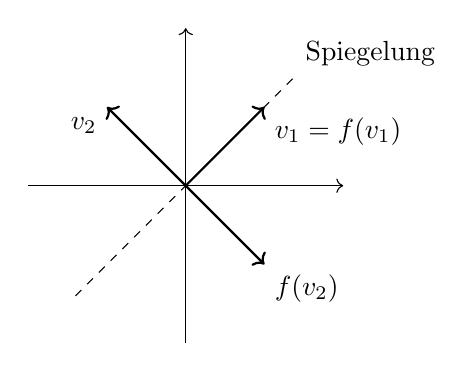
\begin{tikzpicture}
			\draw[->] (-2,0) -- (2,0);
			\draw[->] (0,-2) -- (0,2);
			\draw[dashed] (-1.4,-1.4) -- (1.4,1.4) node[anchor=south west] {Spiegelung};
			\draw[thick,->] (0,0) -- (1,1) node[anchor=north west] {$v_1=f(v_1)$};
			\draw[thick,->] (0,0) -- (-1,1) node[anchor=north east] {$v_2$};
			\draw[thick,->] (0,0) -- (1,-1) node[anchor=north west] {$f(v_2)$};
		\end{tikzpicture}
	Basis $(v_1, v_2)$ aus EVen mit EWen 1, -1, ${_\mathcal B}M_\mathcal B(f) = \twoXtwo{1}{ 0}
																						{0}{-1}$
	\item Drehung um Winkel $0 < \varphi < \pi$.\\
		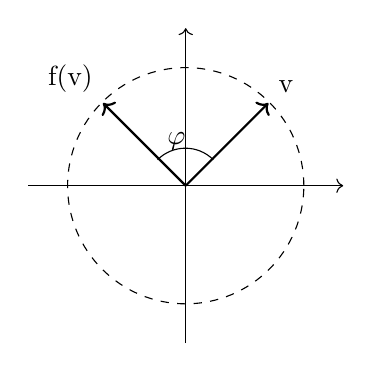
\begin{tikzpicture}
			\draw[->] (-2,0) -- (2,0);
			\draw[->] (0,-2) -- (0,2);
			\draw[dashed] (0,0) circle (1.5cm);
			\draw[thick,->] (0,0) -- (1.05,1.05) node[anchor=south west] {v};
			\draw[thick,->] (0,0) -- (-1.05,1.05) node[anchor=south east] {f(v)};
			\draw (0.35,0.33) arc (45:135:0.5cm) node[anchor=south west] {$\varphi$}; 
			%Es ist perfekt so wie es ist. Zahlen nicht hinterfragen!
		\end{tikzpicture}
	Keinerlei EVen
	\item Scherung \\
	$f(v) = \twoXtwo 	{1} {1}
						{0} {1} v$\\
		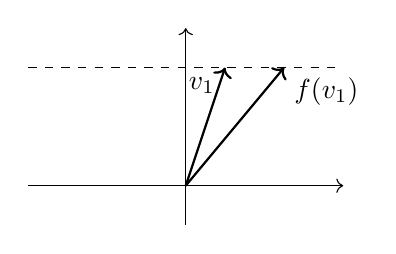
\begin{tikzpicture}
			\draw[->] (-2,0) -- (2,0);
			\draw[->] (0,-0.5) -- (0,2);
			\draw[thick,->] (0,0) -- (0.5,1.5) node[anchor=north east] {$v_1$};
			\draw[thick,->] (0,0) -- (1.25,1.5) node[anchor=north west] {$f(v_1)$};
			\draw[dashed] (-2, 1.5) -- (2, 1.5);

		\end{tikzpicture}		
	EVen nur $\vecTwo	{x}
						{0}$ (mit EW 1), die anderen "scheren aus".
				
\end{enumerate}
\subsection*{Bemerkung}
Ein Vektor $0 \neq v\in V$ ist EV von f zum EW $\lambda$ \\
$\Leftrightarrow v\in ker(f-\lambda\cdot id_V)$. mit $f-\lambda\cdot id_V:V\to V;\tn{ } v \mapsto f(v)-\lambda\cdot v$\\
Also $\lambda$ EW $\Leftrightarrow$ $f-\lambda\cdot id_V$ nicht injektiv.\\
Beweis klar, denn $(f-\lambda\cdot id_V)(v)=0 \Leftrightarrow f(v)-\lambda\cdot v=0$.\\\\
%----------------------------------Vorlesung 8----------------------------------
\textbf{Wdh.:} $f:V\longrightarrow V$ diagonalisierbar $\Leftrightarrow$ es ex. Basis aus EVen.
Wie entscheidet man dies und findet ggf. eine solche Matrix?\\

\subsection*{Definition 4.5.}
Sei $f:V\longrightarrow V$ $K$-Endomorphismus und $\lambda \in K$ (EW von $f$).\\
Dann heißt Eig($f, \lambda$) $:=$ ker($f-\lambda \cdot id_v$) der \textbf{Eigenraum} und dim Eig($f, \lambda$) die \textbf{geometrische Vielfachheit} des EWs $\lambda$.\\
(Also $\lambda$ EW $\Leftrightarrow$ dim Eig($f, \lambda$) $> 0$.)\\
Klar: Eig($f, \lambda$) $\cap$ Eig($f, \mu$) = \{0\} für $\lambda \neq \mu$. Es gilt sogar:
\subsection*{Lemma 4.6.}
Seien $v_1, \dots, v_r$ EVen zu verschiedenen EWen $\lambda_1, \dots, \lambda_r$, so ist \{$v_1, \dots, v_r$\} linear unabhängig.
\subsubsection*{Beweis:}
\begin{tabbing}
Vollständige Induktion über $r$:\\
$r = 1$: nach Definition ist ein EW $v_1 \neq 0$. $\checkmark$\\
$r - 1 \rightsquigarrow r$: \=Seien $v_1, \dots, v_r$ EVen zu verschiedenen EWen $\lambda_1, \dots, \lambda_r$ und gelte\\ \>$\alpha_1 v_1 + \dots + \alpha_r v_r = 0$ mit $\alpha_i \in K$ ($\ast$).\\
\>Dann gilt \=$0 = f(\sum_{i=1}^{r} \alpha_i v_i) = \sum_{i=1}^{r} \alpha_i \lambda_i v_i$ (wende $f$ an)
und\\ \>\>$0 = \sum_{i=1}^{r} \alpha_i \lambda_r v_i$ (multipliziere ($\ast$) mit $\lambda_r$).\\
\>Subtraktion liefert $0 = \alpha_1(\lambda_1 - \lambda_r) v_1 + \dots + \alpha_{r-1} (\lambda_{r-1} - \lambda_r) v_{r-1}$\\ \>$\Rightarrow_{IV} \forall i<r: \alpha_i (\lambda_i - \lambda_r) = 0$\\ \>$\Rightarrow_{\lambda_i \neq \lambda_r} \alpha_i = 0$\\ \>$\Rightarrow_{(\ast)} \alpha_r v_r = 0 \Rightarrow_{v_r \neq 0} \alpha_r = 0.$
\end{tabbing}
Also ist \{$v_1, \dots, v_r$\} linear unabhängig.\\
\subsubsection*{Folgerungen:}
Sei dim $V = n$.
\begin{enumerate}[label=\alph*)]
	\item Jeder $K$-Endomorphismus $f:V\longrightarrow V$ hat höchstens $n$ verschiedene EWe.
	\item Wenn $f$ genau $n$ EWe hat, so ist $f$ diagonalisierbar.\\ (Bed. aber nicht notwendig: Allg. Kriterium folgt.)
\end{enumerate}

\subsection*{Satz 4.7.}
Sei $f:V\longrightarrow V K$-Endomorphismus, $n :=$ dim $V$.\\
Seien $\lambda_1, \dots, \lambda_r$ die verschiedenen EWe von $f$ und $n_i :=$ dim Eig($f, \lambda_i$) deren geometrische Vielfachheit, sowie $\mathcal{B}_i$ Basis von Eig($f, \lambda_i$).
\begin{enumerate} [label = \alph*)]
	\item Es ist $\bigcup_i \mathcal{B}_i$ linear unabhängig, also $\sum_{i} n_i \leq n$.
	\item $f$ diagonalisierbar $\Leftrightarrow \sum_i n_i = n$.
\end{enumerate}

\subsubsection*{Beweis:}
Sei $\mathcal{B}_i = \{v_1^{(i)}, \dots, v_{n_i}^{(i)}\}$.
\begin{enumerate}[label=\alph*)]
	\item Sei $0 = \alpha_1^{(1)} v_1^{(1)} + \dots + \alpha_{n_1}^{(1)} v_{n_1}^{(1)} + \dots + \alpha_1^{(r)} v_1^{(r)} + \dots + \alpha_{n_r}^{(r)} v_{n_r}^{(r)} =: u_1 + \dots + u_r$\\
	mit $u_i \in $ Eig($f, \lambda_i$).\\
	Nach Lemma 4.6. folgt $u_i = 0, \forall i$, da sonst die $u_i \neq 0$ eine Linearkombination von EVen zu verschiedenen EWen wären $\Rightarrow_{\mathcal{B}_i \tn{Basis}} \tn{alle } \alpha_j^{(i)} = 0$.
	\item 
	\begin{itemize}
		\item [--] $"\Leftarrow":$ Dann $\bigcup_i \mathcal{B}_i$ Basis von $V$ aus EVen.
		\item [--] $"\Rightarrow":$ Sei $\mathcal{B}$ Basis aus EVen und sei $m_i$ die Anzahl der EVen in $\mathcal{B}$ zum EW $\lambda_i$.\\
		$\Rightarrow m_i \leq n_i$. Da $n = \sum_i m_i \leq \sum_i n_i \leq_{a)} n \Rightarrow \sum_i n_i = n$.
	\end{itemize}
\end{enumerate}

\subsection*{Vorgehen zur Diagonalisierbarkeit}
\begin{enumerate}[label=\arabic*)]
	\item Finde alle EWe von $f$, d.h. alle $\lambda \in K: f - \lambda\cdot id_V$ nicht injektiv.
	\item Für jeden EW $\lambda_i$ bestimme eine Basis $\mathcal{B}_i$ von Eig($f, \lambda_i$).\\
	$f$ diagonalisierbar $\Leftrightarrow |\bigcup_i \mathcal{B}_i| = n \Leftrightarrow \bigcup_i \mathcal{B}_i$ Basis aus EVen.\\
	Mit Matrizenrechnung: Wähle "Hilfsbasis" $\mathcal{C}$ von $V$ und sei $A := {_\mathcal{C}M_\mathcal{C}}(f)$.\\
	(Oft $f=f_A$, dann $\mathcal{C} = $ Einheitsmatrix.)\\
	Dann gilt:
	\begin{enumerate}
		\item $\lambda \in K \tn{ EW } \Leftrightarrow \tn{rang}(A - \lambda \cdot E) < n \Leftrightarrow \tn{det}(A - \lambda \cdot E) = 0$.
		\item dim Eig($f, \lambda_i$) = dim Eig($A, \lambda_i$) = $n - \tn{rang}(A - \lambda \cdot E)$\\ wobei Eig($A, \lambda$) $:= \{x \in K^n | A \cdot x = \lambda x\}$
	\end{enumerate}
\end{enumerate}

\subsection*{Zusammenhang zwischen Eig($f, \lambda$) und Eig($A, \lambda$)?}
\begin{tabbing}
	\hspace{15pt}\=\hspace{65pt}\=\hspace{2cm}\= \kill
	\>$V \xrightarrow{f (- \lambda id_V)}$ \>$V$\\
	$\Phi{_\mathcal C}$ \>$\uparrow$ \>$\uparrow \Phi_\mathcal C$\\
	\>$K^n \xrightarrow{f_A (- \lambda E)}$ \>$K^n$
\end{tabbing}
Eig($f, \lambda$) = $\Phi_\mathcal C(\tn{ker} f_{A-\lambda E}) = \Phi_\mathcal C(\tn{Eig}(A, \lambda))$, denn \\$0 = (f-\lambda id_V)(v) = \Phi_\mathcal C(f_{A-\lambda E}(\Phi_{\mathcal C}^{-1}(v))) \Leftrightarrow f_{A-\lambda E}(\Phi_{\mathcal C}^{-1}(v)) = 0 \Leftrightarrow \Phi_{\mathcal C}^{-1}(v) \in \tn{ker}(f_{A-\lambda E}) \Leftrightarrow v \in \Phi_{\mathcal C}(\tn{ker}(f_{A-\lambda E}))$.
%----------------------------------Vorlesung 9----------------------------------
\section{Charakteristisches Polynom}
Wiederholung: Sei V K-Vektorraum mit Basis C, $dim(V) = n$ und $f : V \rightarrow V$ ein K-Endomorphismus, $A := {}_{C}M_C(f)$ Ein $\lambda \in K$ ist EW genau dann, wenn \\
$\exists 0 \neq v \in V : f(v) = \lambda \cdot v$\\
$\Leftrightarrow \exists 0 \neq x \in K^n: Ax = \lambda \cdot x$\\
$\Leftrightarrow det(A-\lambda \cdot E) = 0$\\
$P_A := det(X\cdot E - A)$ heißt "charakteristisches Polynom".

\subsection*{Satz 5.1}
$\exists c_0, ... , c_k \in K$ derart, dass \\
$det(\lambda \cdot E - A) = \lambda^n + c_{n-1}\lambda^{n-1} + ... + c_1\lambda + c_0 \forall \lambda \in K.$\\
\subsubsection*{Beweis}
Sei $V:= \lambda \cdot E - A = \left( \begin{matrix}
	\lambda - a_{11} & ... & -a_{1n} \\
	\vdots & \ddots &\vdots \\
	-a_{n1} & ... & \lambda - a_{nn}\\
\end{matrix} \right) $ \\
$\Rightarrow_{\text{Leibnizformel} } det(B) = \sum_{\sigma \in S_n} sgn(\sigma) \prod_{i=1}^{n} b_{i \sigma(i)} = \prod_{i=1}^{n} (\lambda - a_{ii}) + \sum_{\sigma \neq id} sgn(\sigma) \cdot \prod_{i=1}^{n} b_{i \sigma(i)}$, $\forall \sigma \neq id \exists$ höchstens $n-2$ Indizes $i$ mit $\sigma(i) = i,$ Produkt enthält also höchstens $n-2$ mal $\lambda$. \\
$\Rightarrow $ ausmultiplizieren.\\
Spezialfall $n = 2$:
$det\left(\begin{matrix}
	\lambda - a_{11} & -a_{12} \\
	-a_{21} & \lambda - a_{22} \\
\end{matrix}\right) = (\lambda - a_{11})(\lambda - a_{22}) - a_{12}a_{21}$ \\
$=  \lambda^2 - (a_{11} + a_{22}) \lambda + a_{11}a_{22} - a_{12}a_{21} = \lambda^2 - trA\cdot \lambda + det(A)$.\\
mit $trA:= \sum_{i=1}^{n} a_{ii}$ die Spur (englisch "trace") von A.\\
Allgemein gilt $c_{n-1} = -trA$ und $c_0 = (-1)^n detA$ (Übung).\\

\subsection*{Der Polynomring K[X]}
Was ist eigentlich ein Polynom? \\
Idee: formaler Ausdruck $\sum_{i=0}^{n}a_iX^i$ mit $a_i \in K$ - hier $X$ formale Variable \\
versus Polynomfunktion $x \mapsto \sum_{i=0}^{n} a_i x^i , x\in K$ - hier $x$ Körperelement\\
Wiederholung: zu Menge $I$ sei $K^{(I)} := \{ a: I \rightarrow K abb. | \{i \in I | a(i) \neq 0 \} endlich \}$ K-Vektorraum (mit Basis $\{ e_i | i\in I\}$).\\

\subsection*{Definition 5.2}
Sei K ein Körper. Auf $K[X] := K^{(N)}$ sei Ringstruktur definiert via
\begin{itemize}
	\item identifiziere $a_0, a_1, a_2, ...$ mit $\sum_{i=0}^{n}a_i X^i$ (mit $n:= max\{  i | a(i) \neq 0\}$ der Grad $deg(a)$ von $a \neq 0$.)
	\item $(\sum_{i=0}^{n} a_i X^i) + (\sum_{i=0}^{n} b_i X^i) := \sum_{i=0}^{n} (a_i + b_i)X^i , n := max\{deg(a), deg(b)\}$
	\item $(\sum_{i=0}^{n}a_i X^i) \cdot  (\sum_{j=0}^{m} b_j X^j) := \sum_{i=0}^{n} \sum_{j=0}^{m} a_i \cdot b_j \cdot X^{i + j} = \sum_{k = 0}^{m + n}(\sum_{i= 0}^{k} a_i b_{k-i} X^k)$,
\end{itemize}
bezeichnet als Polynomring über K.
\subsubsection*{Bemerkung}
Es ist $K[X]$ kommutativer Ring und "$X$" entspricht $(0,1,0,0,0...)$.\\
Bezeichne $f|g$ "teilt" $g = a\cdot f$ für ein $a \in K[X]$ gilt.

\subsection*{Definition 5.3}
Zu $f = \sum_{i=0}^{n} a\cdot X^i \in K[X]$ und $x \in K$ sei $f(x) := \sum_{i=0}^{n} a_i x^i \in K$ "setze Wert x ein".\\
Es heißt $x \in K$ Nullstelle von $f$, falls $f(x)=0$.\\
\subsubsection*{Bemerkung}
$(f \cdot g)(x) = f(x) \cdot g(x)$.\\

\subsection*{Lemma 5.4}
Zu $p \in K[X]$ und $\lambda \in  K !\exists q\in K[x]$ und $x \in K$ mit $p = q(X-\lambda ) + c$, insbesondere ($\lambda$ einsetzen) ist $\lambda$ Nullstelle von $p \Leftrightarrow X - \lambda | p$.
\subsubsection*{Beweis}
Sei $p = \sum_{i=0}^{n} a_i \cdot x^i$ und $q = \sum_{j=0}^{n-1}b_j x^j$\\
$\Rightarrow a_nX^n + ... + a_1X + a_0 =(b_{n-1}X^{n-1} + ... + b_1X + b_0)(X-\lambda) + c$\\
$= b_{n-1}X^{n} + (b_{n-2} - \lambda b_{n-1})X^{n-1} + ... + (b_0 - \lambda b_1)X-\lambda b_0 + c$\\
genau dann, wenn $b_{n-1} = a_n, b_{n-2} = a_{n-1} + \lambda b_{n-1}, b_0 = a_1 + \lambda b_1, c = a_0 + \lambda b_0$\\
Es gilt $p(\lambda) = 0 \Leftrightarrow c = 0$. \\
Es folgt, dass ein Polynom vom Grad $n$ höchstens $n$ Nullstellen besitzt. \\
(vergleiche Lin.-Alg. I, Blatt 11-4)\\
Wenn auch $q(\lambda) = 0$ ist, so gilt $(X - \lambda)^2 |p$, sage "mehrfache Nullstelle."\\

\subsection*{Definition 5.5}
Zu $A \in Mat_{n\times n}$ sei das Polynom $p_A := det(XE - A) \in K[X]$ das charakteristische Polynom von $A$. (Determinante einer Matrix mit Einträgen im kommutativen Ring $K[X]$). \\
Zu $\lambda \in K$ heißt $m:= max\{i|(X-A)^i|p_A\}$ die algebraische Vielfachheit von $\lambda$. (also $\lambda$ ist EW $\Leftrightarrow m > 0$)

\subsection*{Satz 5.6}
Seien $\lambda_1, .. \lambda_r$ die verschiedenen Eigenwerte der Matrix $A$ und seien $m_i$ bzw. $n_i$ deren algebraische bzw. geometrische Vielfachheit. \\
Dann gilt: $m_i \geq n_i \forall i$. \\
Die Matrix $A$ ist diagonalisierbar,\\
$\Leftrightarrow$
\begin{itemize}
	\item [i.)] $\sum_{i=0}^{r} m_i = n$, d.h. $p_A = \prod_{i=1}^{r} (X- \lambda_i)^{m_i}$. 
	\item [ii.)] $m_i = n_i \forall i$.
\end{itemize}
\subsubsection*{Beweis}
Wähle Basis $v_1, .. v_{n_i}$ zu $Eig(A, \lambda_i)$ und ergänze beliebig zu einer Basis des $K^n$, deren Spalten seien $S$.\\
$\Rightarrow A' = S^{-1}AS = _BM_B(f_A) = \left(
\begin{BMAT}(e)[2pt,3cm,3cm]{ccc.ccc}{ccc.cc}
	\lambda_i & & 0 & & & \\
	& \ddots & & & * & \\
	0 & & \lambda_i & & & \\
	& 0 & & & * & \\
	& & & & & 
\end{BMAT}
\right)$.\\
$\Rightarrow p_A = p_{A'} = (x- \lambda_i)^{n_i} \cdot q \Rightarrow m_i \geq n_i$.\\
$A$ diagonalisierbar $\Leftrightarrow_{\text{Satz 4.7}} \sum_{i=0}^{r}n_i = n$\\
$\Leftrightarrow{\forall n_i \geq m_i} \sum_{i=1}^{r} m_i = m \land \forall i : m_i = n_i$.\\
%----------------------------------Vorlesung 10----------------------------------
\section{Trigonalisierung}
\subsection*{Definition 6.1. }
Matrizen A,B $\in Mat_{nxn}(K)$ heißen \textbf{ähnlich} ($A \approx B$) falls $B=S^{-1}AS$ für ein S $\in GL_n(K)$. Somit ist A diagonalisierbar, falls A ähnlich zu Diagonalmatrix (vgl §4).
\subsection*{Bemerkung}
\begin{enumerate}[label=(\arabic*)]
	\item Ähnlichkeit ist Äquivalenzrelation.
	\item $A\approx A' \Leftrightarrow$ A und A' stellen bzgl. Basen B, B' von V denselben K-Endomorphismus $V \to V$ dar (Satz 4.1).
\end{enumerate}
Was kann man erreichen, wenn A nicht diagonalisierbar ist? \\
\subsection*{Def 6.2.}
Sei $f: V\to V$ ein K-Endomorphismus. Ein Untervektorraum $U \subseteq V$ heißt \textbf{f-invariant} falls $f(U) \subseteq U$. Dann ist $f|_U: U \to U$ wieder K-Endomorphismus. \\
Zum Beispiel ist $U:= Eig(f, \lambda)$ f-invariant: $u\in U \Rightarrow f(u)=\lambda u \in U$. \\
Bezeichne $p_f:= p_A$ mit $A:= {}_{B}M_B(f)$ das charakteristische Polynom von f. (wohldefiniert ist auch $A':= {}_{B'}M_{B'}(f) \Rightarrow A'=S^{-1}AS$ mit $S:={}_{B'}M_B(id_V) \Rightarrow p_{A'}= det(XE-S^{-1}AS) = det(XE - A) = p_A$.
\subsection*{Lemma 6.3}
Ist $U\subseteq V$ f-invariant, so gilt $p_{f|_U} | p_f$.
\subsubsection*{Beweis (vgl. Beweis Satz 5.6.)}
Sei A Basis von U und ergänze zu Basis B von V.
$$\Rightarrow {}_BM_B(f) = 
\left(
\begin{BMAT}(e)[2pt,3cm,3cm]{c.c}{c.c}
	{}_AM_A(f|_U) & * \\
	0 & C  \\
\end{BMAT}
\right) =: \twoXtwo	{A}{B}
					{0}{C}$$ \\
$$\Rightarrow p_f = p_{f|_U} \cdot p_C\tn{, denn }det\twoXtwo	{A}{B}{0}{C} = det\twoXtwo{E}{0}{0}{C}\twoXtwo{A}{B}{0}{E} = detC \cdot detA$$\\
$$\tn{bzw. } det \twoXtwo{XE-A}{-B}{0}{XE-C} = det(XE-A)\cdot det(XE-C)$$
\subsection*{Beispiel}
Die Linksdrehung $f:\mathbb R^2 \to \mathbb R^2$, $\vecTwo{x}{y} \mapsto \vecTwo{-y}{x} = \twoXtwo{0}{-1}{1}{0}\vecTwo{x}{y}$ hat charakteristisches Polynom $p_f = x^2+1 \leadsto$ keine Teiler $q|x^2+1$.\\
$_{\tn{Lemma 6.3.}}\Rightarrow$ es existieren nur triviale invariante Unterräume.
\subsection*{Definition 6.4.}
\begin{enumerate}[label=(\alph*)]
	\item Eine Fahne $(U_j)$ in V ist eine Kette $0 = U_0 \subset U_1 \subset ... \subset U_n = V$ von Unterräumen $U_j$ mit $dim U_j = j$, $\forall j\in \{0,..., n\}$
	\item Ein K-Endomorphismus $f:V\to V$ heißt \textbf{trigonalisierbar}, falls Basis B von V mit $A:= {}_BM_B(f)$ obere Dreiecksmatrix, d.h. $a_{ij}=0$ für $i>j$: $\threeXthree	{*}{ }{*}
																	{ }{\ddots}{ }
																	{0}{ }{*}$
\end{enumerate}										
Matrix heißt \textbf{trigonalisierbar}, falls ähnlich zu oberer Dreiecksmatrix.
\subsection*{Lemma 6.5.}
Ein K-Endomorphismus $f:V\to V$ ist trigonalisierbar gdw. es existiert f-invariante Fahne $(U_j)$ von V, d.h. $f(U_j)\subseteq U_j$, $\forall j$
\subsubsection*{Beweis}
$"\Rightarrow"$ \\
Sei $A:={}_BM_B(f)$ obere Dreiecksmatrix, $B=(v_1,...,v_n)$. \\
Setze $U_j:=span\{v_1,...,v_j\}$ für $j\in \{0,...,n\}$. Eindeutige Fahne. \\
Außerdem: $f(v_j) = \sum_{i\leq j} a_{ij}v_i \in U_j \Rightarrow f(U_j) \subseteq U_j$. \\ \\
$"\Leftarrow"$ \\
Sei  $\{0\} = U_0 \subset U_1 \subset ... \subset U_n = V$ f-invariante Fahne, \\
wähle $(v_1,...,v_n)$ in V mit span $\{v_1,...,v_j\} = U_j$ für $j\in\{0,...,n\}$ d.h. wähle $v_j \in U_j\backslash U_{j-1}$\\
$\Rightarrow$ alle $\{v_1,...,v_n\}$ linear unabhängig $\Rightarrow B=(v_1,...,v_n)$ Basis von V und $f(v_j)\in U_j = span \{v_1,...,v_j\}$ d.h. $f(v_j) = \sum_{i\leq j} a_{ij}v_i \Rightarrow A=(a_{ij})={}_BM_B(f)$ obere Dreiecksmatrix. $\square$
\subsection*{Satz 6.6.}
Ein K-Endomorphismus $f:V\to V$ ist trigonalisierbar gdw. $p_f= \Pi_{i=1}^n(X-\lambda_i)$ zerfällt in Linearfaktoren.
\subsubsection*{Beweis}
$"\Rightarrow"$ \\
Ist $A={}_BM_B(f)$ obere Dreiecksmatrix, so gilt $p_f = p_A = det(XE-A) = \Pi_{i=1}(X-a_{ii}).$\\ \\
$"\Leftarrow"$ \\
Induktion nach n. I.A. n=1: klar. \\
I.S. n-1 $\leadsto$ n: Es existiert EW $\lambda_1$ von f, wähle dazu EV $v_1$ und ergänze zu Basis B=($v_1,w_2,...,w_n)$ und $W:= span\{w_2,..., w_n\}$. \\
$$A:= {}_BM_B(f) = 
\left(
\begin{BMAT}(e)[2pt,3cm,3cm]{c.ccc}{c.ccc}
	\lambda_1 & a_{12} & ... & a_{1n} \\
	0 & & & \\
	\vdots & & B &  \\
	0 & & & 
\end{BMAT}
\right)
\tn{, sei } 
\begin{array}{l}
	g:W\to W, \\
	w_j \mapsto \sum_{i=2}^na_{ij}w_i \\
	\tn{(NB: W nicht notwendigerweise f-invariant)}
\end{array}
$$
$\Rightarrow p_f = (X-\lambda_1)\cdot p_g$ und $p_g$ zerfällt $\Rightarrow$ es existiert g-invariante Fahne 
$\{0\} = W_0 \subset W_1 \subset ... \subset W_{n-1}= W$ \\
Setze $V_1 := KV_1$ und $U_j := V_1 + W_{j-1}$ für $j\in\{0,...,n\}$ ($\Rightarrow dimU_j = 1+ dim W_{j-1}=j$)\\
$\Rightarrow \{0\} = U_0 \subset U_1 \subset ... \subset U_n = V$ Fahne und f-invariant: \\
$$
f(\alpha v_1+w)\lambda_1 \alpha v_1+cv_1+g(w)\in V_1 + W_{j-1} = U_j\tn{ (mit }c\in K).
$$
\subsection*{Beispiel}
$A:= \threeXthree{1}{-1}{0}{-1}{1}{-2}{-2}{2}{-2}$, $p_A = (X-1)^2(X+2)+4+4(X-1)-(X+2)=X^3$. 
Einziger EW 0, aber A nicht diagonalisierbar denn geometrische Vielfachheit = 1. \\
Setze EV $v_1:= \vecThree{1}{1}{0}$, $B_1=(v_1, e_2, e_3)$, $J_1:= {}_{B_1}M_A(id) = \threeXthree{1}{1}{0}{1}{0}{0}{0}{0}{1}$, $J^{-1}_1AJ_1 = \threeXthree{0}{-1}{-2}{0}{2}{2}{0}{-2}{-2}$ \\
$B:= \twoXtwo{2}{2}{-2}{-2}$ hat $p_B = X^2$, EV $\vecTwo{-1}{1}$, $B_2'=(\vecTwo{-1}{1}, e_1)$, \\ $S:=\twoXtwo{-1}{1}{1}{0}$, $J_2:=\left( 
\begin{matrix}
	1 & \begin{matrix} 0 & 0 \end{matrix} \\
	\begin{matrix} 0 \\ 0 \end{matrix} & S\\
\end{matrix}
\right)$, $J:=J_1\cdot J_2 \Rightarrow J^{-1}AJ = \threeXthree{0}{-1}{-1}{0}{0}{-2}{0}{0}{0}$ obere Dreiecksgleichung.
%----------------------------------Vorlesung 11----------------------------------
\section*{Einschub: Komplexe Zahlen}
\subsection*{Definition 6.7.}
\begin{tabbing}
	Auf $\mathbb{C} := \mathbb{R}^2$ sei \=Addition $(a, b) + (a', b') := (a+a', b+b')$ und\\
	\>Multiplikation $(a, b) \cdot (a', b') := (aa'-bb', ab'+a'b)$ definiert.\\ (wobei $a, b, a', b' \in \mathbb{R}$); diese Struktur heißt Körper der \textbf{komplexen Zahlen}.
\end{tabbing}
Körperaxiome leicht nachzuprüfen, $(a, b)^{-1} = (\frac{a}{a^2+b^2}, \frac{-b}{a^2+b^2})$.\\
Identifiziere $\mathbb{R} \longrightarrow \mathbb{C}, a \longmapsto (a, 0)$\\ und setze $i := (0,1) \Rightarrow i^2 = -1$ und $(a, b) = a+bi$.\\
Zu $z = a+bi \in \mathbb{C}$ sei $a\in\mathbb{R}$ \textbf{Realteil}, $b\in\mathbb{R}$ \textbf{Imaginärteil} und $\bar{z} := a - bi \in \mathbb{C}$ die \textbf{konjugiert} komplexe Zahl.\\
\subsection*{Bemerkung}
Für $z, w \in \mathbb{C}$ gilt $\overline{z+w} = \bar{z}+\bar{w}$ und $\overline{zw} = \bar{z} \cdot \bar{w}$.\\
\subsection*{Geometrische Anschauung}
Addition = Vektoraddition\\
Multiplikation: multipliziere Beträge, addiere "Winkel" ($\leadsto$ Analysis)\\
zu $z = a+bi\in\mathbb{C}$ sei $|z| := \sqrt{a^2+b^2} = \sqrt{z\cdot \bar{z}}$ der \textbf{Betrag}, $|zw| = |z| \cdot |w|$.\\
\begin{figure}[h]
	\begin{tikzpicture}
		\tkzInit[xmax=4,ymax=4]
		\tkzDrawXY[noticks,>=latex,/tkzdrawX/label=Re,/tkzdrawY/label=Im]
		\draw[thick,-latex] (0,0) -- (1,1) node[anchor=north west] {$1+i$};
		\draw[thick,-latex] (0,0) -- (2,1) node[anchor=north  west] {$2+i$};
		\draw[thick,-latex] (0,0) -- (1,3) node[anchor=north west] {$1+3i$};
		\tkzText[left](-2,2){$(2+i)(1+i) = 1+3i$}
	\end{tikzpicture}
\end{figure}
\subsection*{Satz 6.8. "Fundamentalsatz der Algebra"}
Jedes Polynom $p\in\mathbb{C}[X]$ zerfällt in Linearfaktoren.\\
Beweis z.B. Funktionentheorie
\section*{Cayley-Hamilton}
\subsection*{Definition 6.9.}
Sei $f:V\longrightarrow V$ ein $K$-Endomorphismus und $p=\sum_{i=0}^{n}c_iX^i\in K[X]$ ein Polynom. Dann sei $p(f) := \sum_{i=0}^{n}c_if^i:V\longrightarrow V$ wieder $K$-Endomorphismus, wobei $p(f)(v) = \sum_{i=0}^{n}c_if^i(v)$ für $v\in V$, wobei $f^i(v) = \underbrace{f( \dots (f}_{i-mal}(v))\dots)$, $f^0:=id_V$.\\
Für $f=f_A$ mit $A\in$ Mat$_{n\times n}(K)$ sei $p(A) := \sum_{i=0}^{n}c_iA^i$, also $f_{p(A)} = p(f_A)$.\\
Erinnerung: Zu $f:V\longrightarrow V K$-Endomorphismus $p_f := p_A := det(X\cdot E - A)$, $A := {_B}M_B(f)$.\\
\subsection*{Satz 6.10. (Cayley-Hamilton)}
Es gilt $p_f(f)=0$, insbesondere $p_A(A)=0$.
\subsubsection*{Beweis:}
Elementarer Beweis via Begleitmatrizen:
\subsection*{Definition 6.11.}
Zu $p = X^n+c_{n-1}X^{n-1}+\dots+c_1X+c_0\in K[X]$ sei\\
$A :=
\left(\begin{matrix}
	0 & & & -c_0\\
	1 & \ddots & & \colon\\
	 & \ddots & 0 & \colon\\
	 & & 1 & -c_{n-1}
\end{matrix}\right)$ die \textbf{Begleitmatrix} zu $p$.\\
Es gilt $p_A = p$ (Übung).\\
(Es ist leicht $p_A(A)e_1 = 0$ einzusehen.)\\
$\Rightarrow$ $\sum c_iA^ie_1 = c_0e_1+c_1e_2+\dots+c_{n-1}e_n+(-c_0e_1-\dots-c_{n-1}e_n)$\\\\
\textbf{Vorbemerkung.} Sei $f:V\longrightarrow V$ ein $K$-Endomorphismus, $0\neq v\in V$ sowie $1 \leq r \leq n$ maximal mit $\{v, f(v), \dots, f^{r-1}(v)\}$ linear unabhängig.\\
Dann: \begin{enumerate}[label=\alph*)]
	\item $f^r(v)\in U := \tn{span}\{v, \dots, f^{r-1}(v)\}$,
	\item $U$ ist $f$-invariant,
	\item mit $f^r(v) + \sum c_if^i(v) = 0$ ist $p_{f|_U} = X^r+\sum c_iX^i$,
	\item $p_{f|_U}(f)(v) = 0$.
\end{enumerate}
\subsubsection*{Beweis:}
\begin{enumerate}[label=\alph*)]
	\item Wegen $\{v, f(v), \dots, f^r(v)\}$ linear abhängig klar.
	\item $f(f^i(v)) = f^{i+1}(v)\in U$ f.a. $i \in \{0, \dots, r-1\}$
	\item $\mathcal{B} := (v, f(v), \dots, f^{r-1}(v))$ Basis und ${_\mathcal{B}}M_{\mathcal{B}}(f|_U) = \left(\begin{matrix}
		0 & & & -c_0\\
		1 & \ddots & & \colon\\
		& \ddots & 0 & \colon\\
		& & 1 & -c_{n-1}
	\end{matrix}\right)$ Begleitmatrix.
\item $p_{f|_U}(f)(v) = f^r(v)+\sum_{i=0}^{r-1}c_if^i(v) = 0.$
\end{enumerate}
\subsection*{Beweis (Satz):}
Zeige $p_f(f)(v) = 0$ f.a. $0\neq v \in V$. Sei $U$ wie in Vorbemerkung\\
$\Rightarrow_{Lemma 6.3.} p_f = p_c \cdot p_{f|_U}$ für ein Polynom $p_c \in K[X]$\\
$\Rightarrow p_f(f) = p_c(f) \circ p_{f|_U}(f)$\\
$\Rightarrow p_f(f)(v) = p_c(f)(\underbrace{p_{f|_U}(f)(v)}_{=0\tn{ nach Vorbem.}}) = 0$.
\subsection*{Beispiel:}
$A:= \left(\begin{matrix}
	3 & 0 & -1\\
	1 & 2 & -1\\
	-1 & 1 & 1
\end{matrix}\right), p_A = \tn{det}\left(\begin{matrix}
X-3 & 0 & 1\\
-1 & X-2 & 1\\
1 & -1 & X-1
\end{matrix}\right) = X^3-6X^2+11X-6$\\
$A^2=\left(\begin{matrix}
	10 & -1 & -4\\
	6 & 3 & -4\\
	-3 & 3 & 1
\end{matrix}\right), A^3 = \left(\begin{matrix}
33 & -6 & -13\\
25 & 2 & -13\\
-7 & 7 & 1
\end{matrix}\right)$\\
$A^3-6A^2+11A-6E = \left(\begin{matrix}
	33 & -6 & -13\\
	25 & 2 & -13\\
	-7 & 7 & 1
\end{matrix}\right) - \left(\begin{matrix}
60 & -6 & -24\\
36 & 18 & -24\\
-18 & 18 & 6
\end{matrix}\right) + \left(\begin{matrix}
33 & 0 & -11\\
11 & 22 & -11\\
-11 & 11 & 11
\end{matrix}\right) - \left(\begin{matrix}
6 & 0 & 0\\
0 & 6 & 0\\
0 & 0 & 6
\end{matrix}\right) = 0$\\
\subsection*{Alternative Beweisskizze:}
Es ex. Körper $K \subset L$ derart, dass $p_f$ über $L$ zerfällt (Bew. Algebra + Zahlentheorie).\\
Über $L$ ist $f$ nach Satz 6.6. trigonalisierbar.\\
Ist $A' = S^{-1}AS$, so gilt $p(A') = S^{-1}p(A)S$.\\
Ohne Einschränkung $A = \left(\begin{matrix}
	\lambda_1 &  & *\\
	 & \ddots & \\
	0 & & \lambda_n
\end{matrix}\right)$ und $p_A = \prod_{i=1}^{n}(X-\lambda_i)$.\\
Zeige direkt $p_A(A) = \prod_{i=1}^{n}(A-\lambda_iE) = 0$.
%----------------------------------Vorlesung 12----------------------------------
\section{Jordan-Normalform}
\subsection*{Definition 7.1}
Sei V ein n-dim. K-VR und $U_1, ..., U_r \subseteq V$ UVR.\\
Schreibe $U_1 \oplus ... U_r \subseteq V$,
falls $\sum_{i=1}^{r} u_i = 0$, wobei  $u_i \in U_i \Rightarrow$ alle $u_i = 0$\\
($\Leftrightarrow u_j \cap \sum_{i \neq j}u_i = {0}  \forall j$).\\
Falls zusätzlich $U_1 + ... + U_r = V$, schreibe $V = U_1 \oplus ... \oplus U_r$, sage direkte Summe.
\subsubsection*{Beispiel}
\begin{itemize}
\item[-]
$B = (v_1, ..., v_n)$ Basis $\Rightarrow V = Kv_1 \oplus ... \oplus Kv_n$.
\item[-]
Sei $f: V \rightarrow V$ ein K-Endomorphismus und $\lambda_1 , ... , \lambda_r \in K$ verschiedene Eigenwerte von $f \Rightarrow  \bigoplus_{i=1}^{r} \underbrace{Eig(f, \lambda_i)}_{:= ker(f-\lambda \cdot id_v)} \subseteq
 V$ mit $"="$ gdw. f diagonalisierbar.(vgl. Satz 4.7)
\end{itemize}
\subsection*{Definition 7.2}
Zu $ f: V \rightarrow V$ K-Endomorphismus sei $VEig(f, \lambda) := \{ v \in V | (f - \lambda \cdot id_v)^s(v) = 0 \text{für ein} s \in \mathbb{N} \}\supseteq Eig(f, \lambda)$ verallgemeinerter Eigenraum, auch "Hauptraum".
\subsection*{Beispiel}
$A = 
\left( \begin{matrix}
	3 & 5 \\
	0 & 4 \\
\end{matrix} \right),
p_a = (X-3)^2$\\
$Eig(A,3) = span{\left(\begin{matrix}
		1 \\
		0 \\
	\end{matrix}\right)}, VEig(A,3) = K^2$, da $(A-3\cdot I)^2 = 0$.
\subsection*{Bemerkung 7.3}
Sei $g:= f - \lambda \cdot id_v \in EndV.$ betrachte Ketten\\ 
${0} \subseteq kerg \subseteq kerg^2$ ...\\
$V \supseteq img \supseteq img^2$...\\
Es gilt $dim kerg^i + dim img^i = n \forall i (*).$\\
Sei $s (\leq n)$ minimal mit $kerg^s = kerg^{s+1} \Rightarrow_{(*)} img^s = im g^{s+1}$\\
 und es gilt $kerg^s = kerg^{s+i}, img^s = img^{s+i} \forall i$.\\
Denn $g^{-1}(kerg^k) = kerg^{k+1}, g(img^k) = img^{k+1}$.
\subsection*{Lemma 7.4}
Sei $g:= f - \lambda \cdot id_v \in EndV$ und sei $s$ minimal mit $kerg^s = kerg^{s+1}$\\
, also $U:= VEig(f, \lambda) = kerg^s$.\\
Dann ist $W:= img^s$ komplementär zu $U$, d.h. $V = U \oplus W$.\\
Weiterhin sind $U$ und $W$ jeweils f-invariant.
\subsubsection*{Beweis}
$gW = g(img^s) = img^{s+1} = img^s = W \Rightarrow g^sW = W$\\
$\Rightarrow g^s|_W \in EndW$ ist surjektiv, also injektiv.\\
$\Rightarrow W \cap = W \cap kerg^s = \{ 0 \} \Rightarrow_{\text{Bemerkung (*)}} V = U\oplus W$.\\
Da $W$ $g$-invariant ist es auch $f = g + \lambda \cdot id_v$-invariant.\\
Ebenso ist $U$ $g$-invariant: \\
Sei $u\in U$, $g^s(u) = 0$
$\Rightarrow g^s(g(n)) = g^{s+1}(n) = 0 \Rightarrow g(u) \in U$.\\
Mit Basis $B = (\underbrace{u_1, ..., u_k}_{\in U}, \underbrace{w_1, ..., w_l}_{\in W})$ ist ${}_{B}M_{B} = \left( \begin{matrix}
	* & 0 \\
	0 & *\\ 
\end{matrix} \right)$.\\
\subsection*{Lemma 7.5}
Sei $\lambda \neq \mu \Rightarrow VEig(f, \lambda) \cap VEig(f, \mu) = \{0\}$.\\
Der einzige EW von $f|U$ ist $\lambda$ , wobei $U := VEig(f, \lambda)$.
\subsubsection*{Beweis}
Zuerst "$VEig(f,\lambda) \cap Eig(f, \mu) = \{0\}$"($\Rightarrow$ 2. Aussage).\\
Sei $v\in Eig(f, \mu)$\\
$\Rightarrow (f-\lambda \cdot id)v = (\mu - \lambda)v$\\
$\Rightarrow (f-\lambda \cdot id)^sv = (\mu - \lambda)^sv \forall s \in \mathbb{N}$.\\
Also $v\in U \Rightarrow (\mu - \lambda)^sv = 0 \Rightarrow v = 0$.\\
Jetzt sei $v \in VEig(f,\mu)$ und $v\in U$, sei s min. $(f-\mu \cdot id)^sv = 0,$ ang. $s > 0$\\
$\Rightarrow (f-\mu \cdot id)^{s-1} \in Eig(f,\mu) \cap U = \{0\}$ (da $U f$-invariant).\\
$\Rightarrow (f-\mu \cdot id)^{s-1}v = 0$ im Widerspruch zu $s$ minimal.
\subsection*{Satz 7.6 (Hauptraumzerlegung)}
Sei $f \in EndV$ und sei $p_f = \prod_{i=i}^{r}(X-\lambda_i)^{m_i}$ mit verschiedenen EW $\lambda_i$.\\
Dann \begin{enumerate}[label=(\alph*)]
	\item $dim VEig(f,\lambda_i) = m_i$(algebraische Vielfachheit)
	\item $V = \bigoplus_{i=1}^{r} VEig(f, \lambda_i)$.
\end{enumerate}
\subsubsection*{Beweis}
\begin{enumerate}[label=(\alph*)]
	\item $\lambda = \lambda_i$, sei $U := VEig(f,\lambda)$ und $W$ wie in Lemma 7.4.\\
	$\Rightarrow p_f = p_{f|U}\cdot p_{f|W}$ und beide zerfallen in Linearfaktoren.\\
	$\Rightarrow_{\text{Lemma 7.5}} p_{f|U} = (X-\lambda)^{dim_u}, p_{f|W}(\lambda) \neq 0 \Rightarrow m_i = dimU$.\\
	\item  Induktion über $dimV$, sei $\lambda = \lambda_1$.
	IV auf $f|W$ ergibt $V = U \oplus \bigoplus_{j = 1}^{s} VEig(f|W, \mu_j)$.\\
	Die $\mu_j sind die \lambda_i \neq \lambda_1$.\\
	Zeige noch $VEig(f,\mu) \subseteq W$ für die $\mu = \mu_j$.\\
	Sei $v \in V$ mit $(f-\mu \cdot id)^sv = 0$, schreibe $v = u + w \in U \oplus W$.\\
	$\Rightarrow_{U, W f-invariant} (f- \mu \cdot  id)^su = 0 \Rightarrow_{\text{Lemma 7.5}} u = 0 \Rightarrow v = w \in W$.
\end{enumerate}
\subsection*{Beispiel}
$A = \left( \begin{matrix}
	1 & -3 & -2\\
	-4 & 0 & 2\\
	2 & -6 & -4\\
\end{matrix} \right), 
p_A = det\left( \begin{matrix}
	X-1 & 3 & 2\\
	4 & X & -2\\
	-2 & 6 & X+4\\
\end{matrix} \right) \\
= X(X-1)(X+4) + 12 + 48 + X + 12(X-1) - 12(X+4) = X^2(X+3)$\\
$Eig(A,-3) = span\{ \left( \begin{matrix}
	1 \\
	0 \\
	2 \\
\end{matrix}\right)\}$\\
$Eig(A,0) = span\{ \left( \begin{matrix}
	1 \\
	-1 \\
	2 \\
\end{matrix}\right)\}$\\
$A^2 =\left( \begin{matrix}
	9 & 9 & 0 \\
	0 & 0 & 0 \\
	18 & 18 & 0 \\
\end{matrix}\right) \leadsto VEig(A,0) = span\{ 
\left( \begin{matrix}
1 \\
-1 \\
2 \\
\end{matrix} \right) ,
\left( \begin{matrix}
0 \\
0 \\
1 \\
\end{matrix} \right) \}$\\
Mit $S := 
\left( \begin{matrix}
	1 & 0 & 1 \\
	-1 & 0  & 0 \\
	2 & 1 & 2 \\
\end{matrix} \right)$ folgt $S^-1AS = 
\left( \begin{matrix}
	0 & -2 & \\
	& 0 \\
	 & & -3 \\
\end{matrix}\right)$ \\
%----------------------------------Vorlesung 13----------------------------------
\subsection*{}
Sei $f:V \rightarrow V$ ein K-Endomorphismus mit $p_f = \prod_{i = 1}^{r}(X-\lambda_i)^{m_i}$.\\
Nach Satz 7.6 (Hauptraumzerlegung) ist 
$V = \bigoplus_{i=1}^{r}V_i$ mit $V_i := VEig(f, \lambda_i), dim V_i = m_i$.\\
Mit Basis $B = (\underbrace{v_1^1, ... , v_{m_1}^1}_{\in V_1}, ... , \underbrace{v_1^r, ... , v_{m_r}^r}_\in V_r)$ ist ${}_BM_B(f) = \left( \begin{matrix}
	* & 0 \\
	0 & * \\
\end{matrix}\right)$ (Blockgestalt) und für jedes $i$ ist $(f-\lambda \cdot id)|_{v_i}$ nilpotent.
\subsection*{Bezeichnung}
$J_k := \left( \begin{matrix}
	0 & 1 \\
	& \ddots & \ddots \\
	& & \ddots& 1 \\
	& & & 0 \\
\end{matrix} \right) \in Mat_{k \times k}(K)$ Jordanmatrix. $J_k^k = 0.$\\
Zu $g \in EndV$ nilpotent sei $s$ minimal mit $g^s = 0$ der Nilpotenzindex. Also $k$ im Fall $J_k$.
\subsection*{Proposition 7.7}
Sei $dim_kV = n$ und sei $g\in EndV$ mit Nilpotenzindex $s$. Dann existiert Basis $B$ von $V$ und $s = s_1 \leq ... \leq s_l$ mit $\sum_{j=1}^{l}s_j = n$ und $l = dim ker g$, sodass $\left( \begin{matrix}
	J_{s_1} \\
	& \ddots \\
	& & J_{s_l}\\
\end{matrix} \right)$.\\
Die $s_1, ..., s_l$ sind eindeutig bestimmt.
\subsubsection*{Beweis}
Sei $U_i := kerg^i \Rightarrow \{0\} = U_0 \subset U_1 \subset ... \subset U_{s-1} \subset U_s = V$.\\
Wegen $g(v) \in U_{i-1} \Leftrightarrow v\in U_i$ gilt: $U_i \subseteq U_{s-1}$.\\
Wähle $W_s \subseteq V mit V =  U_{s-1} \oplus W_s \Rightarrow g(W_s) \subseteq U_{s-1}$.\\
Zeige $"g(W_s) \cap U_{s-2} = \{0\}"$: \\
Sei $w\in W_s$ und $v := g(w) \in U_{s-2} \Rightarrow g^{s-1}(w) = 0 \Rightarrow w\in U_{s-1} \Rightarrow w = 0 \Rightarrow v = 0.\checkmark$\\
Wähle $W_{s-1} \subseteq U_{s-1}$ mit $U_{s-1} = U_{s-2} \oplus W_{s-1}$ und $g(W_s) \subseteq W_{s-1}$.\\
Erhalte so $V = U_s = U_{s-1} \oplus W_s = U_{s-2} \oplus W_{s-1} \oplus W_s = ... = (U_0 \oplus)W_1 \oplus ... \oplus W_s$\\
mit $W_i \cap U_{i-1} = \{0\} \forall i > 1$, insbesondere $W_i \cap kerg = \{0\}$.\\
Somit ist $g|w_i : W_i \rightarrow W_{i-1}$ injektiv, erhalte $W_S \rightarrow_g W_{s-1} \rightarrow_g ... \rightarrow_g W_1$.\\
Wähle Basis $w_1^s, ... , w_{k_s}^s$ von $W_s$\\
$g(w_1^s), ..., g(w_{k_s}^s), w_1^{s-1}, ..., w_{k_{s-1}}^{s-1}$ von $W_{s-1}$\\
$\vdots$\\
$g^{s-1}(w_1^s), ... , g^{s-1}(w_{k_s}^s), g^{s-2}(w_1^{s-1}), ..., g^{s-2}(w_{k_{s-1}}^{s-1}), ..., w_1^1, ..., w_{k_1}^1$ von $W_1 = U_1$\\
und ordne spaltenweise von unten nach oben.\\
$\Rightarrow {}_BM_B(g) =$ Blockdiagonale $(\underbrace{J_s, ... J_s}_{k_s \text{mal}} , \underbrace{J_{s-1}, ... , J_{s-1}}_{k_{s-1} \text{mal}}, ..., \underbrace{J_1, ..., J_1}_{k_1 \text{mal}})$\\
und Anzahl Blöcke ist $l = dimU_1 = dimkerg$.\\
Dabei ist $dimW_i$ und die $k_s, ..., k_1$ durch $dimU_i$, also $g$ eindeutig bestimmt.\\
\subsection*{Beispiel}
$B := \left( \begin{matrix}
0 & 1 & 3 \\
0 & 0 & 2 \\
0 & 0 & 0 \\
\end{matrix} \right),
B^2 = \left(\begin{matrix}
0 & 0 & 2 \\
0 & 0 & 0 \\
0 & 0 & 0 \\
\end{matrix}\right),
B^3 = 0 \Rightarrow s=3$ \\
$\{0\} \subset U_1 span\{ \left( \begin{matrix}
1 \\
0 \\
0 \\
\end{matrix}\right) \} \subset U_2 = span\{ \left(\begin{matrix}
1\\
0\\
0\\

\end{matrix}\right) , \left( 
\begin{matrix}
0\\
1\\
0\\
\end{matrix}\right) \} \subset K^3$\\
$\Rightarrow V = U_2 \oplus span\{ \left(\begin{matrix}
0\\
0\\
1\\
\end{matrix}\right)\} = U_1 \oplus span\{ \left(\begin{matrix}
3\\
2\\
0\\
\end{matrix}\right)\} \oplus W_3 = (U_1 \oplus) span\{\left(\begin{matrix}
2\\
0\\
0\\
\end{matrix}\right)\} \oplus W_2 \oplus W_3$, mit $g(W_3) \subseteq W_2$ und $g(W_2) \subseteq W_1$(hier gleich)\\
$\Rightarrow S := \left(\begin{matrix}
	2 & 3 & 0\\
	0 & 2 & 0\\
	0 & 0 & 1\\
\end{matrix}\right) ergibt S^{-1}BS = \left(\begin{matrix}
0 & 1 \\
& 0 & 1\\
& & 0\\
\end{matrix}\right), g^2(v) g(w) v = \left(\begin{matrix}
0\\
0\\
1\\
\end{matrix}\right)$\\
Aus Satz 7.6 und Proposition 7.7 folgt:
\subsection*{Satz 7.8(Jordan-Normalform)}
Sei $f\in EndV$ mit $p_f = \prod_{i = 1}^{r}(x-\lambda_i)^{m_i}$ in Linearfaktoren. Dann existiert Basis $B$ mit ${}_BM_B(f) = \left(\begin{matrix}
	A_1 \\
	& \ddots \\
	& & A_r\\
\end{matrix}\right)$, wobei jedes $A_i = \lambda_i E_{m_i} + \left(\begin{matrix}
J_{s_1^i} \\
& \ddots \\
& & J_{s_{l_i}^i}
\end{matrix}\right).\\$
Man nennt $\left(\begin{matrix}
\lambda & 1 \\
& \ddots & \ddots \\
& & \ddots & 1\\
& & &  \lambda \\
\end{matrix}\right) = J_k + \lambda E_k$ auch Jordanblock zu $\lambda$.\\
Die Jordanblöcke sind bis auf Reihenfolge eindeutig.\\
Zum EW $\lambda_i$ ist \begin{itemize}
	\item Anzahl Jordanblöcke $= dimEig(f,\lambda_i)$(geometrische Vielfachheit)
	\item größter Jordanblock $\stackrel{\wedge}{=}$ Nilpotenzindex
\end{itemize}
FAZIT: Die Jordansche Normalform (JNF) löst das eindeutige Repräsentantenproblem für Ähnlichkeit von Matrizen in $\mathbb{C}$. (Zwei Matrizen sind ähnlich $\Leftrightarrow$ JNF ist gleich)
%----------------------------------Vorlesung 14----------------------------------
\section{Euklidische Vektorräume}
\subsection*{Erinnerung (Lin Alg I, Ausblick)}
Zu $x, y \in \mathbb{R}^n$ sei ${\skalar{x}{y}} := \sum_{i=1}^{n}x_iy_i$ "Standardskalarprodukt"\\
$\parallel x\parallel := \sqrt{\skalar{x}{x}}$ "Norm"\\
$x \perp y \Leftrightarrow {\skalar{x}{y}} = 0$

\subsection*{Definition 8.1.}
Sei $V$ ein reeller Vektorraum. Eine Abbildung $\genskalar: V \times V \longrightarrow \mathbb{R}$ heißt \textbf{Skalarprodukt} falls gilt:
\begin{enumerate}
	\item [--] (S1): ${\skalar{\lambda v + \mu v'}{w}} = \lambda {\skalar{v}{w}} + \mu {\skalar{v'}{w}}\\
	{\skalar{v}{\lambda w + \mu w'}} = \lambda {\skalar{v}{w}} + \mu {\skalar{v}{w'}}$ (bilinear)
	\item [--] (S2): ${\skalar{v}{w}} = {\skalar{w}{v}}$ (symmetrisch)
	\item[--] (S3:) ${\skalar{v}{v}} \geq 0$ und ${\skalar{v}{v}} = 0 \Leftarrow v = 0$ (positiv definit)
\end{enumerate}

(f.a. $v, w, v', w' \in V, \lambda, \mu \in \mathbb{R}$).
Ein $\mathbb{R}$-Vektorraum mit Skalarprodukt ($V$, $\genskalar$) heißt \textbf{euklidischer Vektorraum}.

\subsection*{Bemerkung}
\begin{enumerate} [label=\arabic*)]
	\item \begin{itemize}
		\item ${\skalar{0}{w}} = {\skalar{0v}{w}} = 0{\skalar{v}{w}} = 0$ entsprechend ${\skalar{v}{0}} = 0$
		\item (S2) und linear in 1. oder 2. Komponente $\Rightarrow$ (S1)
		\item (S1) und ${\skalar{v}{v}} > 0$ f.a. $v \neq 0 \Rightarrow$ (S3)
	\end{itemize}
	\item Im $V = \mathbb{R}^n$ ist ${\skalar{x}{y}} := \sum_{i=1}^{n}x_iy_i$ ein Skalarprodukt.\\
	\begin{itemize}
		\item (S2) $\checkmark$
		\item (S1) $({\skalar{\lambda x+\mu x'}{y}} =)\sum_{i=1}^{n}(\lambda x_i+\mu x'_i)y_i = \lambda\sum_{i=1}^{n}x_iy_i+\mu\sum_{i=1}^{n}x'_iy_i (= \lambda{\skalar{x}{y}}+\mu{\skalar{x'}{y}})$
		\item (S3) $\sum_{i=1}^{n}x_i^2 \geq 0 \checkmark$ und $\sum_{i=1}^{n}x_i^2 = 0 \Rightarrow$ alle $x_i^2 = 0 \Rightarrow \tn{ alle } x_i^2 = 0$
	\end{itemize}
\end{enumerate}

\subsection*{Satz 8.2. (Cauchy-Schwarz'sche Ungleichung)}
Sei $(V, \genskalar)$ euklidischer Vektorraum und seien $v, w \in V$\\
$\Rightarrow {\skalar{v}{w}}^2 \leq {\skalar{v}{v}} \cdot {\skalar{w}{w}}$.

\subsubsection*{Beweis:}
Ansatz $0 \leq {\skalar{v+\lambda w}{v+\lambda w}} =_{\tn{(S1), (S2)}} {\skalar{v}{v}}+2\lambda {\skalar{v}{w}}+\lambda^2{\skalar{w}{w}}$\\
(o.E. $w \neq 0$) $\Rightarrow_{\tn{(S3)}} 0 \leq \frac{\skalar{v}{v}}{\skalar{w}{w}}+2\lambda \frac{\skalar{v}{w}}{\skalar{w}{w}}+\lambda^2 = (\lambda + \frac{\skalar{v}{w}}{\skalar{w}{w}})^2-\frac{\skalar{v}{w}^2}{\skalar{w}{w}^2}+\frac{\skalar{v}{w}}{\skalar{w}{w}}$\\
Wähle $\lambda := -\frac{\skalar{v}{w}}{\skalar{w}{w}} \Rightarrow \frac{\skalar{v}{w}^2}{\skalar{w}{w}^2} \leq \frac{\skalar{v}{v}}{\skalar{w}{w}}$\\
$\Rightarrow {\skalar{v}{w}}^2 \leq {\skalar{v}{v}} \cdot {\skalar{w}{w}}$.
\subsection*{Bezeichnung}
$\parallel v \parallel := \sqrt{\skalar{v}{v}}$ die \textbf{Norm} von $v \in V$, dann (CSU): $|\skalar{v}{w}| \leq \parallel v\parallel \cdot \parallel w\parallel$.
\subsection*{Corollar 8.3.}
Die Abbildung $\parallel \cdot \parallel: V \longrightarrow \mathbb{R}$ erfüllt:
\begin{enumerate}[label=\alph*)]
	\item $\norm{v} \geq 0$ und $\norm{v} = 0 \Leftrightarrow v = 0$
	\item $\norm{\lambda v} = |\lambda|\cdot \norm{v}$
	\item $\norm{v+w} \leq \norm{v}+\norm{w}$ (Dreiecksungleichung)
\end{enumerate}
(f.a. $v, w \in V, \lambda \in \mathbb{R}$).
\subsubsection*{Beweis:}
\begin{enumerate}[label=\alph*)]
	\item (S3) $\checkmark$
	\item ${\skalar{\lambda v}{\lambda v}} = \lambda^2{\skalar{v}{v}}$ wg. (S1) $\checkmark$
	\item $\eskalar{v+w}^2 = {\skalar{v+w}{v+w}} = {\skalar{v}{v}}+2{\skalar{v}{w}}+{\skalar{w}{w}}\\ \leq_{\tn{CSU}} \norm{v}^2 + 2\norm{v}\cdot\norm{w}+\norm{w}^2 = (\norm{v}+\norm{w})^2$.
\end{enumerate}

\subsection*{Definition 8.4.}
Zu ($V, \genskalar$) euklidischer Vektorraum und $0 \neq v, w \in V$,\\ definiere $\alpha \in [0, \pi]$ mit $cos \alpha = \frac{\skalar{v}{w}}{\norm{v}\cdot\norm{w}}$ ($\in_{\tn{CSU}} [-1, 1]$)
\textbf{Winkel} $\sphericalangle(v, w)$ zwischen $v, w$.
\newpage
\subsubsection*{Begründung:}
\begin{figure}[h]
	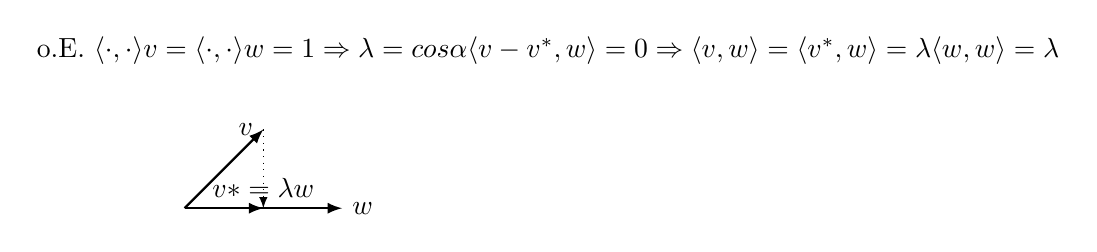
\begin{tikzpicture}
		\tkzInit[xmax=3,ymax=3]
		\draw[thick,-latex] (0,0) -- (1,1) node[anchor=east] {$v$};
		\draw[thick,-latex] (0,0) -- (2,0) node[anchor=west] {$w$};
		\draw[dotted,-latex] (1,1) -- (1,0);
		\draw[thick,-latex] (0,0) -- (1,0) node[anchor=south] {$v* = \lambda w$};
		\tkzText[right](-2,2){o.E. $\genskalar{v} = \genskalar{w} = 1 \Rightarrow \lambda = cos\alpha\\{\skalar{v-v^*}{w}} = 0\\\Rightarrow {\skalar{v}{w}} = {\skalar{v^*}{w}} = \lambda {\skalar{w}{w}} = \lambda$}
	\end{tikzpicture}
\end{figure}

Weiterer Beispiele für Skalarprodukte:
\begin{enumerate}[label=\arabic*)]
	\item $V = \mathbb{R}[X]^{< n} := \{\sum_{i=0}^{n-1}a_iX^i | a_i \in \mathbb{R}\}$\\
	Wähle $x_1, \dots, x_n \in \mathbb{R}$ verschieden, ${\skalar{f}{g}} := \sum_{i=1}^{n}f(x_i)g(x_i)$\\
	(S1), (S2) $\checkmark$\\
	(S3): ${\skalar{f}{f}} = \sum_{i=1}^{n}f(x_i)^2 \geq 0$\\
	und $\sum_{i=1}^{n}f(x_i)^2 = 0 \Rightarrow \tn{ alle } f(x_i) = 0 \Rightarrow_{\tn{deg}f<n} f = 0$\\
	Entsprechende Beispiele aus der Analysis:\\
	$V = C[0,1] := \{f:[0,1] \longrightarrow \mathbb{R} \tn{ stetig}\}\\
	{\skalar{f}{g}} := \int_{0}^{1}f(x)g(x)dx$
	\item $V = \mathbb{R}^n$, sei $A \in \tn{Mat}_{n\times n}(\mathbb{R})$ und setze ${\skalar{v}{w}} := v^TAw = \sum_{i, j=1}^{n}a_{ij}v_iw_j$.\\
	(S1): $(\lambda v+\mu v')^TAw = \lambda v^TAw+\mu v'^TAw$\\
	analog für $w$.\\
	(S2)?: $w^TAv = v^TA^Tw = v^TAw$ f.a. $v, w \in V \Leftrightarrow A^T = A$ (da $e_i^TAe_j=a_{ij}$)\\
	(S3)?: gdw. $v^TAw > 0$ f.a. $v \neq 0$ "positiv definite Matrix" $\rightsquigarrow$ später
\end{enumerate}
%----------------------------------Vorlesung 15----------------------------------
\subsection*{Bemerkung}
Ist $(V, \genskalar)$ euklidischer Vektorraum und $U \subseteq V$ ein Untervektorraum, so ist auch $\genskalar_U:U\times U \to \mathbb R$ (Einschränkung) Skalarprodukt. \\
Sei nun $(V, \genskalar)$ euklidischer VR und sei $U \subseteq V$ Untervektorraum.
\subsection*{Definition 8.5.} Zu $v\in V$ heißt $v^*\in U$ Bestapproximation von V in U falls $||v-v^*||$ kleinstmöglich ist, d.h. $||v-v^*|| \leq ||v-u||$, $\forall u \in U$
\subsection*{Proposition 8.6.}
Es ist $v^* \in U$ Bestapproximation von v $\Leftrightarrow \skalar{v-v^*}{u} = 0$, $\forall u \in U$. \\
Falls eine Bestapproximation existiert, so ist sie eindeutig.
\subsection*{Bemerkung}
Sei $u \in U$. $||v-v^*+u)||^2 = || v-v^*||^2-2\skalar{v-v^*}{u} + ||u||^2$. \\
Falls $\skalar{v-v^*}{u} = 0$ folgt $||v-(v^*+u)|| \geq ||v-v^*||^2$. Also $||v-v^*|| \leq ||v-u'||$, $.\forall u'\in U$. \\
Umgekehrt sei $v^*$ Bestapproximation $\Rightarrow ||v-(v^*+\lambda u)||^2 = ||v-v^*||^2-2\lambda\skalar{v-v^*}{u} + \lambda^2||u||^2 \geq ||v-v^*||^2 \Rightarrow 2\lambda\skalar{v-v^*}{u} \leq \lambda^2||u||^2$, $\forall \lambda \in \mathbb R_{>0} \Rightarrow \skalar{v-v^*}{u} = 0$. \\
Außerdem $||v-(v^*+u)||^2 > ||v-v^*||^2$ falls $u \neq 0$ $\Rightarrow$ Eindeutigkeit der Bestapproximation
\subsection*{Definition 8.7} 
Sei $(V, \genskalar)$ euklidischer Vektorraum. Eine Basis $S \subseteq V$ heißt Orthonormalbasis falls $\skalar{e}{f} = \twopartdef{1}{\tn{falls }e = f}{0}{\tn{sonst}}$ für $e,f \in S$. \\
Im Fall $S= \{v_1,...,v_n\}$ also $\skalar{v_i}{v_j} = \delta_{ij} = \twopartdef{1}{\tn{falls } i=j}{0}{\tn{sonst}}$.
\subsection*{Bemerkung}
Angenommen U (wie oben) hat ONB $\{u_1,...,u_k\}$, $k = dim U$. \\
Dann setze $v^*:= \sum_{i=1}^k\skalar{v}{u_i}u_i$. \\
Dies ist Bestapproximation nach Proposition 8.6. \\
Denn: Sei j beliebig $\Rightarrow \skalar{v^*}{u_j} = \sum_{i=1}^k\skalar{v}{u_i}\skalar{u_i}{u_j} = \skalar{v}{u_j} \Rightarrow \skalar{v-v^*}{u_j} = 0$.
Somit $\skalar{v-v^*}{u} = 0$, $\forall u \in U$. \\
Diese Bemerkung ist die Grundlage für folgendes wichtiges Resultat.
\subsection*{Satz 8.8}
Sei $(V, \genskalar)$ euklidischer Vektorraum und $v_1,..., v_n \in V$ linear unabhängig. Dann existiert $u_1,...,u_n \in V$ mit $\skalar{u_i}{u_j} = \delta_{ij}$ und $span \{u_1,...,u_j\} = span \{v_1,..., v_j\}$, $\forall j$. \\
Insbesondere hat jeder endlich-dim. euklidischer VR eine Orthonormalbasis.
\subsection*{Bemerkung}
"Gram-Schmidt'sches Orthonormalisierungsverfahren" \\
Induktion/n. $n=1$: $u_1 := \frac{v_1}{||v_1||}$ \\
$n \leadsto n+1$: Sei $u_1,..., u_n$ ONB von $U:=span\{v_1,...,v_n\}$. \\
Dann ist $v_{n+1} \notin U$. Betrachte $v^*_{n+1} := \sum_{i=1}^n \skalar{v_{n+1}}{u_i}u_i$ Bestapproximation in U, sei $v_{n+1}' := v_{n+1} - v^*_{n+1}$, $u_{n+1} := \frac{v_{n+1}'}{||v_{n+1}'||}$. \\
Dann gilt $\skalar{u_{n+1}}{u_j} = 0$, $\forall j \leq n$, \\
sowie $span \{u_1,...,u_{n+1}\} = span \{v_1,...,v_{n+1}\}$
\subsection*{Definition 8.9}
Zu  $(V, \genskalar)$ euklidischer Vektorraum und $U \subseteq V$ UVR sei $U^\perp := \{v\in V| \skalar{v}{u}=0, \forall u\in U\}$ Orthogonalraum (ist auch UVR). Also $v^*\in U$ Bestapproximation $\Leftrightarrow v-v^* \in U^\perp$. \\
Sei nun U endlich-dim. mit ONB $u_1,...,u_k$ und betrachte $p:V\to V$, $v \mapsto v^*:= \sum_{i=1}^k\skalar{v}{u_i}u_i \Rightarrow p\in EndV$. Es gilt $p^2=p$, $imp = U$, $v-p(v)\in U^\perp$ "Orthogonalprojektion".
\subsection*{Bemerkung}
$ker p = U^\perp$. Da: $"\subseteq" v\in kerp \Rightarrow v=v-p(v)\in U^\perp$ \\
$"\supseteq" v \in U^\perp \Rightarrow \skalar{v}{u_i} = 0\forall i \Rightarrow p(v)=0$.
\subsection*{Proposition 8.10.}
Ist U endlich-dim. so $V=U\oplus U^\perp$.
Ist auch V endlich-dim. so $U = (U^\perp)^\perp$.
\subsubsection{Beweis}
Sei $p\in EndV$ Orthogonalprojektion auf U, wie oben $\Rightarrow p^2=p \Rightarrow V=ker p \oplus im p$ (vgl. Blatt 4, Aufgabe 4) $\Rightarrow_{\tn{Bemerkung}} V = U^\perp \oplus U$. \\
Sei $dimV = n \Rightarrow dim U^\perp = n - dim U$.
Da stets U $\subseteq (U^\perp)^\perp$ gilt (trivial) folgt $U = (U^\perp)^\perp = n- dim U^\perp = n - (n- dimU) = dim U$ 
%----------------------------------Vorlesung 16----------------------------------
\section{Selbstadjungierte Endomorphismen}
Für die Theorie der Endomorphismen von euklidischen VRen benötigen wir auch Skalarprodukte über $\mathbb C$. \\
Für $x,y\in \mathbb C$ definiere $\skalar{x}{y}:= \sum_{i=0}^{n}x_i\bar{y_i}$ Standardskalarprodukt. \\
Dann $\skalar{x}{x} = \sum_{i=0}^{n}|x_i|^2$ und $\norm{x} := \sqrt{\skalar{x}{x}}$ wie vorher.
\subsection*{Definition 9.1.}
Sein V ein komplexer VR. Eine Abbildung $\genskalar:V\times V\to \mathbb C$ heißt Skalarprodukt falls gilt: \\
\begin{enumerate}[start=1,label={(\bfseries S\arabic*)':}]
	\item $\skalar{\lambda v+\mu v'}{w} = \lambda\skalar{v}{w} + \mu \skalar{v'}{w}$ \\
 	$\skalar{v}{\lambda w+\mu w'} = \bar\lambda\skalar{v}{w} + \bar\mu\skalar{v}{w'}$ (sesquilinear)
	\item $\skalar{w}{v}=\overline{\skalar{v}{w}}$ (konjugiert symmetrisch)
	\item $\skalar{v}{v} \geq 0$ und $\skalar{v}{v} = 0 \gdw v = 0$ (positiv definit)
\end{enumerate}
Man nennt $(V,\genskalar)$ einen unitären VR.
\subsection*{Bemerkung}
\begin{enumerate}
	\item Linearität in 1. Komponente + (S2)' $\Rightarrow$ (S1)'
	\item $\skalar{v+\lambda w}{v+\lambda w} = \skalar{v}{v} + \lambda\skalar{w}{v} \bar\lambda\skalar{v}{w} + \skalar{w}{w} = \skalar{v}{v} + 2Re(\bar\lambda\skalar{v}{w})+|\lambda|^2\skalar{w}{w}$
	Es folgt wie vorher die Cauchy-Schwarz'sche Ungleichung:
		$$0 \leq |\lambda|^2 + 2Re\bar\lambda\frac{\skalar{v}{w}}{\skalar{w}{w}} + \frac{\skalar{v}{v}}{\skalar{w}{w}} = \left( \lambda + \frac{\skalar{v}{w}}{\skalar{w}{w}}\right)\left( \bar\lambda + \frac{\overline{\skalar{v}{w}}}{\skalar{w}{w}}\right) - \left| \frac{\skalar{v}{w}}{\skalar{w}{w}}\right|^2 + \frac{\skalar{v}{v}}{\skalar{w}{w}}\tn{, } \forall  \lambda\in\mathbb C\tn{.}$$
		$$\Rightarrow \left| \frac{\skalar{v}{w}}{\skalar{w}{w}}\right|^2 \leq \frac{\skalar{v}{v}}{\skalar{w}{w}}
		\Rightarrow |\skalar{v}{w}|^2 \leq \eskalar{v} \eskalar{w} \tn .$$
	\item Charakterisierung der Bestapproximation $v^*$ von v in U wie vorher via $v-v^*\perp u$, $\forall u\in U$. \\
	(Ist $v^*$ Bestapproximation $\Rightarrow 2Re \bar\lambda\skalar{v-v^*}{u} \leq |\lambda|^2 \norm{u}^2$, $\forall \lambda\in\mathbb C$ wähle $\lambda := \frac{\skalar{v-v^*}{u}}{|\skalar{v-v^*}{u}|}\cdot\mu$ mit $\mu > 0$.... $\Rightarrow |\skalar{v-v^*}{u}|= 0$.)
	\item Ist $u_1,...,u_k\in U$ ONB, so ist $v^*=\sum_{i=1}^{k}\skalar{v_i}{u_i}u_i$ Bestapprox. \\
	Es folgt Gram-Schmidt-Orthonormalisierung wie vorher.
\end{enumerate}	
\subsection*{Lemma 9.2.}
Sei V ein endl.-dim. K-VR mit Skalarprodukt $(K=\mathbb R)$ oder $K=\mathbb C$. Zu $\varphi:V\to K$ linear existiert genau ein $y_\varphi\in V$ mit $\varphi \skalar{\cdot}{y-z}$, d.h. $\varphi = \skalar{x}{y_\varphi}$, $\forall x\in V$.
\subsection*{Bemerkung}
\subsubsection*{"Eindeutigkeit"}
Gelte $\skalar{\cdot}{y} = \skalar{\cdot}{z} \Rightarrow \skalar{\cdot}{y-z}=0$, insbesondere $\eskalar{y-z}=0 \Rightarrow_{(S3)} y=z$.
\subsubsection*{"Existenz"}
Sei $(v_1,...v_n)$ eine ONB von V. Dann finde $y_\varphi=\sum_{i=1}^{n}\lambda_iv_i$ mit $\varphi(v_i)=\skalar{v_i}{y_\varphi} = \skalar{v_i}{\sum_{j=1}^{v_j}} = \sum_{j=1}^{n} \lambda_j \skalar{v_i}{v_j} = \overline\lambda_i$, also setze $\lambda_i := \overline{\varphi(v_i)} \Rightarrow \varphi(\sum_{j=1}^{n}\lambda_iv_i) = \skalar{\sum_{i=1}^{n}\lambda_iv_i}{y_\varphi}$.
\subsection*{Definition 9.3.}
Sei $f:V\to W$ ein Homomorphismus zwischen VRen mit Skalarprodukt. Dann heißt $f^*:W\to V$ Homomorphismus zu f adjungiert, falls 
$$\skalar{f(v)}{w} \skalar{v}{f^*(w)}\tn{, } \forall v\in V,w\in W\tn .$$
D.h. $f^*(w)$ ist so, dass $V\to K,v\mapsto \skalar{f(v)}{w}$ von der Form $\skalar{\cdot}{f^*(w)}$ ist. \\
Ist V endl.-dim. so existiert stets $f^*$.
\subsection*{Definition 9.4.}
Ein Endomorphismus $f:V\to V$ heißt selbstadjungiert falls $\skalar{f(v)}{w} = \skalar{v}{f(w)}$, $\forall v,w\in V$. \\
Das heißt $f=f^*$. Speziell sei $f_A:K^n\to K^n,x\mapsto A\cdot x$ (Standardskalarprodukt), dann $\skalar{Ax}{y} = \skalar{x}{Ay} \gdw x^TA^T\overline y = (Ax)^T\overline y = x^T(\overline{Ay}) = x^T\overline A\overline y \gdw A^T = \overline A$ "Hermite'sche Matrix", symmetrische Matrix falls $K=\mathbb R$
\subsection*{Satz 9.5.}
Jeder EW eines selbstadjungierten Endomorphismus ist reell.
\subsubsection*{Beweis}
Sei $0\neq v\in V$ ein EV zum EW $\lambda$ von $f:V\to V$.
$$\Rightarrow \lambda \eskalar{v} = \skalar{\lambda v}{v} = \skalar{f(v)}{v} = \skalar{v}{f(v)} = \skalar{v}{\lambda v} = \overline\lambda\eskalar{v} \Rightarrow_{\eskalar{v}\neq 0} \lambda = \overline\lambda$$
%----------------------------------Vorlesung 17----------------------------------
Ziel: Jeder selbstadjungierte Endomorphismus ist diagonalisierbar ( via ONB).\\
Bezeichnung: $\left. \begin{array}{l}
	$Euklidischer VR über $\mathbb{R}\\
	$Unitärer VR über $\mathbb{C}\\
\end{array}\right\}$ "VR mit Skalarprodukt" über $K=\mathbb{R}\tn{ oder } \mathbb{C}$.\\

\subsection*{Lemma 9.6.}
Sei $V$ VR mit Skalarprodukt und $f \in \tn{End}(V)$ selbstadjungiert. Dann sind EVen zu verschiedenen EWen orthogonal.
\subsubsection*{Beweis:}
Sei $f(v)=\lambda v, f(w) = \mu w$ mit $v, w\neq 0, \lambda \neq \mu$\\
$\Rightarrow_{\tn{Satz 9.5.}} \lambda, \mu\in\mathbb{R}.$
$\transp{\lambda\skalar{v}{w} = \skalar{\lambda v}{w} = }$ $\skalar{f(v)}{w} = \skalar{v}{f(w)} \transp{= \skalar{v}{\mu w} = \mu \skalar{v}{w}}$\\
$\Rightarrow_{\lambda \neq \mu} \skalar{v}{w} = 0$. $\Box$\\\\
Wie sieht die Matrix von $f:V\longrightarrow W$ bezüglich ONBen aus?\\
Seien $\mathcal{B}=(v_1, \dots, v_n) \tn{ und } \mathcal{C} = (w_1, \dots, w_n)$ ONBen von $V, W$.\\
$\Rightarrow$ Koordinaten-Isomorphismus $\Phi^{-1}:W\longrightarrow K^m$ ist $w\longmapsto\underbrace{(\skalar{w}{w_i})_i}_{\transp{\skalar{\sum_{j=1}^{n}\lambda_jw_j}{w_i} = \lambda_i}}$\\
$\Rightarrow A = (a_{ij}) = {_{\mathcal{B}}}M_{\mathcal{C}}(f)$ mit $a_{ij}=\skalar{f(v_j)}{w_i}$.\\
Ist $f\in\tn{End}(V)$ selbstadjungiert, so ist $a_{ij} = \skalar{f(v_j)}{v_i} = \skalar{v_j}{f(v_i)} = \overline{a_{ji}}$,\\
d.h. $A = (a_{ij}) = {_\mathcal{B}}M_{\mathcal{B}}(f)$ ist Hermite'sch.
\subsection*{Proposition 9.7.}
Ist dim$V$ endlich, so besitzt jeder selbstadjungierte Endomorphismus $f\in\tn{End}(V)$ einen reellen EW.
\subsubsection*{Beweis:}
Sei $\mathcal{B}$ ONB von $V$ und $A:={_{\mathcal{B}}}M_{\mathcal{B}}(f)\in \tn{Mat}_{n \times n}(K)\\
\Rightarrow A \tn{ Hermite'sch und } p_A\in \mathbb{C}[X] \tn{ hat eine Nullstelle } \lambda \in \mathbb{C}$\\
(d.h. $f_A:\mathbb{C}^n\longrightarrow\mathbb{C}^n \tn{ selbstadjungiert, hat EV in } \mathbb{C}^n$).\\
$\Rightarrow_{\tn{Satz 9.5.}} \lambda \in \mathbb{R}$\\
$\Rightarrow p_A\in K[X] \tn{ hat Nullstelle in } \mathbb{R}$
$$\tn{d.h. } f_A:\mathbb{R}^n\longrightarrow\mathbb{R}^n \tn{ hat EV in } \mathbb{R}^n, \tn{ falls } K=\mathbb{R}. \Box$$
\subsection*{Satz 9.8.}
Sei $V$ ein endlich-dimensionaler VR mit Skalarprodukt und sei $f\in \tn{End}(V)$ selbstadjungiert. Dann existiert ONB $\mathcal{B}$ von $V$ mit ${_{\mathcal{B}}}M_{\mathcal{B}}(f)$ reelle Diagonalmatrix.
\subsubsection*{Beweis:}
Induktion/dim$V$. Nach Prop. 9.7. existiert EW $\lambda \in \mathbb{R}$ von $f$.\\
Sei $0\neq U:=\tn{Eig}(f, \lambda)$ und wähle ONB $(u_1, \dots, u_k)$ von $U$\\
$\Rightarrow f(U) \subseteq U.$ Zeige $f(U^{\perp}) \subseteq U^\perp.$ Sei $w \in U^\perp, u\in U$\\
$\Rightarrow \skalar{u}{f(w)} =_{\transp{f \tn{ selbstadj.}}} \skalar{\underbrace{f(u)}_{\in U}}{w} = 0.$\\
Betrachte $g:=f|_{U^\perp} \in \tn{End}(U^\perp)$, auch selbstadjungiert.\\
$\Rightarrow_{\tn{IV.}} \tn{ existiert ONB} (u_{k+1}, \dots, u_n) \tn{ von } U^\perp$ s. d. g reell diagonalisiert.\\
$\Rightarrow \mathcal{B}:=(u_1, \dots, u_m) \tn{ ONB von } U \oplus U^\perp = V \tn{ und } {_{\mathcal{B}}}M_{\mathcal{B}}(f) = \left(\begin{matrix}
	\lambda & & & & & \\
	 & \ddots & & & & \\
	 & & \lambda & & & \\
	 & & & \lambda_{k+1} & & \\
	 & & & & \ddots & \\
	 & & & & & \lambda_n\\
\end{matrix}\right). \Box$
\subsection*{Definition 9.9.}
Eine Matrix $\begin{matrix}O\\U\end{matrix} \in \tn{Mat}_{n \times n}\vecTwo{\mathbb{R}}{\mathbb{C}}$ heißt $\begin{matrix}\tn{\textbf{orthogonal}}\\\tn{\textbf{unitär}}\end{matrix}$ falls $O^TO=E$ bzw. $U^*U=E$, wobei $U^*:= \overline{U}^T$.
\subsection*{Corollar 9.10.}
Jede $\begin{matrix}\tn{symmetrische}\\\tn{Hermite'sche}\end{matrix}$ Matrix $A \in \tn{Mat}_{n \times n}(K)$ hat eine $\begin{matrix}\tn{orthogonale}\\\tn{unitäre}\end{matrix}$ Matrix $\begin{matrix}O\\U\end{matrix}$ s.d. $\begin{matrix}O^TAO\\U^*AU\end{matrix}$ reelle Diagonalmatrix ist.
\subsubsection*{Beweis:}
\begin{tabbing}
	\hspace{15pt}\=\hspace{45pt}\=\hspace{2cm}\= \kill
	\>$K^n \xrightarrow{f_A}$ \>$K^n$\\
	$\transp{f_O}$ $\tn{ }\Phi{_\mathcal B}$ \>$\uparrow$ \>$\uparrow \Phi_\mathcal B \transp{\downarrow f_O^{-1}}$\\
	\>$K^n \xrightarrow{f_D}$ \>$K^n$
\end{tabbing} wähle Spalten von $\begin{matrix}O\\U\end{matrix}$ als ONB $\mathcal{B}$ wie in Satz 9.8.\\
$\Rightarrow O^{-1}AO = D, U^{-1}AU = D$\\[10pt]
$\begin{matrix}e_i^TO^TOe_j = (Oe_i)^T(Oe_j) = S_{ij}\\e_i^TU^*Ue_j = (Ue_i)^*(Ue_j) = S_{ij}\end{matrix} \Rightarrow \begin{matrix}O^TO\\U^*U\end{matrix} = E. \Box$\newpage
\textbf{Verfahren:}
\begin{enumerate}[label=\arabic*)]
	\item Die Eigenräume berechnen.
	\item Jeweils ONB finden (falls dim Eig $> 1$).
\end{enumerate}
%----------------------------------Vorlesung 18----------------------------------
\section{Isometrien und normale Endomorphismen}
Erinnerung: Ein Skalarprodukt definiert geometrische Größen
$\norm{v} = \skalar{v}{v}^{\frac{1}{2}}$(Länge), $cos\angle(v,w) := \frac{\skalar{v}{w}}{\norm{v}\cdot \norm{w}}$(Winkel)$K = \mathbb{R}$.
\subsection*{Definition 10.1}
Eine lineare Abbildung $f: V \longrightarrow W$ zwischen VR mit Skalarprodukt heißt Isometrie, falls $\skalar{f(v)}{f(w)} = \skalar{v}{w} \forall v,w \in V$.\\
\subsection*{Bemerkung}
\begin{enumerate}[label = \alph*)]
	\item Isometrien sind stets injektiv.
	\item Isometrien erhalten Längen, Winkel, Orthogonalität
	\item $V = W = \mathbb{R}^2: A = \left( \begin{matrix}
		cos(\alpha) & -sin(\alpha) \\
		sin(\alpha) & cos(\alpha) \\
	\end{matrix}\right)$ Drehung um $\alpha$.\\
	oder $A = \left( \begin{matrix}
		cos(\alpha) & sin(\alpha) \\
		sin(\alpha) & -cos(\alpha) \\
	\end{matrix}\right)$ Achsenspiegelung.
\end{enumerate}
Ein System $S\subseteq V$ heißt Orthonormalsystem (ONS), falls $\skalar{v}{w} = \twopartdef{0}{\text{falls } v \neq w}{1}{\text{falls } v = w} (v,w\in S).$ D.h. ONB ist erzeugendes ONS.
\subsection*{Lemma 10.2}
Sei B ONB von $V$ und $f: V \longrightarrow W$ linear.\\
Dann $f$ Isometrie $\Leftrightarrow f(B)$ ist ONS und $f$ injektiv.
\subsubsection*{Beweis}
$"\Rightarrow"$\\
$\skalar{f(v)}{f(w)} =_{\text{f Iso.}} \skalar{v}{w} =_{\text{ONB}}  \twopartdef{0}{\text{falls } f(v) \neq f(w)}{0}{\text{falls } f(v) = f(w)}$(da $f$ injektiv).\\
$"\Leftarrow"$\\
Seien $v = \sum_{i}\lambda_i u_i, w= \sum_{j} \mu_j u_j$ mit $u_i, u_j \in B$\\
$\Rightarrow \skalar{f(v)}{f(w)} = \sum_{i, j} \lambda_i\bar\mu_j \skalar{f(u_i)}{f(u_j)} =_{f(B)\text{ ONS}, B \text{ ONS}} \sum_{i,j}\lambda_i\bar\mu_j \skalar{u_i}{u_j}$
\subsection*{Lemma 10.3}
Sei $f: V \longrightarrow W$ mit adj. Abb. $f^* : W \longrightarrow V$. Dann $f$ Isometrie $\Leftrightarrow f^* \circ f = id_v$.
\subsubsection*{Beweis}
$\skalar{f^*(f(v))}{w} = \skalar{f(v)}{f(w)} \forall v,w \in V.$\\
Seien $B, C$ ONB von $V, W$ (endlich-dim.) und $A:= {}_BM_C(f), A^* := {}_CM_B(f^*).$
Dann $f$ Isometrie $\Leftrightarrow A^*A = E$.
\subsection*{Bemerkung}
Eine surjektive Isometrie $f: V \longrightarrow W$ ist ein VR-Isomorphismus.\\
In dem Fall $B$ ONB $\Rightarrow f(B)$ONB.\\
Falls $dimV = dimW < \infty$ ist jede Isometrie surjektiv.\\
Für $f: V\longrightarrow V$ und ONB $B$ von $V$ ist dann $A := {}_BM_B(f) \begin{matrix}
	\text{"orthogonal"} (K = \mathbb{R})\\
	\text{"unitär"} (K = \mathbb{C})\\
\end{matrix}$ denn $A^*A = E$.
\subsection*{Definition 10.4}
Sei V VR mit Skalarprodukt.\\
$Iso(V) := \{f:V\longrightarrow V | f \text{ surj. Isometrie}\}$ ist die Isometriegruppe von $(V, \skalar{\cdot}{\cdot})$.\\
\subsection*{Bemerkung}
Sind $f,g \in Iso(V)$, so auch $f\circ g, f^{-1} \in Iso(V)$.\\
Speziell $(V = K^n)$ heißt\\
$O(n) := \{O \in Mat_{n\times n}(\mathbb{R} | O^TO = E)\}$ orthogonale, \\
$U(n) := \{U \in Mat_{n\times n}(\mathbb{C} | U^*U = E)\}$ unitäre Gruppe. ("Untergruppen" von $GL_n(K)$.)
\subsection*{Bemerkung}
\begin{enumerate}[label = \alph*)]
	\item Ist $\lambda$ EW von $f \in Iso(V)$, so gilt $|\lambda| = 1$.
	\item $detO = \pm 1 , |detU| = 1$ 
\end{enumerate}
(Eine Abbildung $f_O$ mit $detO = 1$ heißt "orientierungstreu").
\subsection*{Beispiel}
Was sind die Isometrien des $\mathbb{R}^3$?\\
Sei $f\in Iso(\mathbb{R}^3) \Rightarrow p_f$(Grad 3) hat eine Nullstelle $\lambda_1$.\\
Sei $u_1$ EV (mit $\norm{u_1} = 1$) zu $\lambda_1 \in  \{1, -1\}$ und ergänze zu ONB $B = (u_1, u_2, u_3)$\\
$\Rightarrow U:= span\{u_2,u_3\}$ erfüllt $f(U) = U$, denn $U = span\{u_1\}^{\perp}$ und $f$ erhält Orthogonalräume von f-inv. Unterräumen.\\
$\Rightarrow {}_BM_B(f) = \left(\begin{BMAT}(e)[2pt,3cm,3cm]{c.ccc}{c.ccc}
	\lambda_1 & 0 & & 0 \\
	0 & & & \\
	& & A^{'} & \\
	0 & & & 
\end{BMAT}\right) =: A$ und $f|_U \in Iso(U), det(A) = \lambda_i det(A^{'})$\\
Falls $det(A^{'}) = -1 \leadsto f|_U$ Achsenspiegelung $\Rightarrow$ zwei EW $1, -1,$kann $u_2, u_3$ als EV wählen.
Falls $det(A^{'}) = 1 \leadsto f|_U$ Drehung.\\
Die orientierungstreuen Isometrien sind Drehungen um eine Achse.
%----------------------------------Vorlesung 19----------------------------------
\subsection*{Definition 10.5.}
Ein Endomorphismus $f:V\to V$ heißt normal falls $f^*f = ff^*$ gilt, d.h. $\skalar{f^*(f(v))}{w} = \skalar{f(f^*(v))}{w}$, $\forall v,w\in V$. \\
Sei B ONB von V und $A:={}_BM_B(f)$, $A^*={}_BM_B(f^*)$, so bedeutet dies $A^*A=AA^*$ "normale" Matrix.
\subsection*{Bemerkung}
\begin{enumerate}[label=\alph*)]
	\item Jeder selbstadjungierter oder orthogonale unitäre Endomorphismus normal
	\item Ist f normal, so gilt $kerf^*=ker f$.
\end{enumerate}
\subsection*{Lemma 10.6.}
Sei $f\in End(V)$ normal.
\begin{enumerate}[label=\alph*)]
	\item Für $\lambda\in K$ gilt $Eig(f,\lambda) Eig(f^*,\overline\lambda)$
	\item Sind $\lambda\neq\mu$ EWe mit EVen v,w, so gilt $\skalar{v}{w}=0$.
\end{enumerate}
\subsubsection*{Beweis}
\begin{enumerate}[label=\alph*)]
	\item Es gilt $(f-\lambda id)^*=f^*-\overline\lambda\cdot id$ und auch $f-\lambda\cdot id$ ist normal $\Rightarrow ker(f-\lambda\cdot id) = ker(f^*-\overline\lambda\cdot id)$.
	\item $\skalar{f(v)}{w} = \skalar{\lambda v}{w} = \lambda\skalar{v}{w}$ \\
	$\skalar{f(v)}{w} = \skalar{v}{f^*(w)} = \skalar{v}{\overline\mu w} = \mu\skalar{v}{w} \Rightarrow_{\lambda + \mu} \skalar{v}{w} = 0$
\end{enumerate}
\subsection*{Satz 10.7. (Spektralsatz)}
$K=\mathbb C$. \\
$f\in End(V)$ normal $\gdw$ es existiert ONB aus EVen Matrixfrom: $A \in Mat_{nxn}(\mathbb C)$ normal $\gdw U^*AU = D$ diagonal für U unitär (sage: A ist "unitär diagonalisierbar").
\subsubsection*{Beweis}
$"\Leftarrow"$ \\
Sei $(v_1,...,v_n)$ ONB mit $f(v_i) = \lambda v_i$ $\Rightarrow f^*(v_i) = \overline\lambda_iv_i \Rightarrow f^*(f(v_i)) = f^*(\lambda_iv_i) = \overline\lambda_i\lambda_iv_i = \lambda_i\overline{\lambda_i}v_i = f(\overline\lambda_iv_i) = f(f^*(v_i)) \Rightarrow f^*f = ff^*$. \\
$"\Rightarrow"$ \\
Vollständige Induktion $n:=dimV$. n=1 klar. \\
$n-1 \leadsto n$: Sei $\lambda$ ein EW von f (existiert da K=$\mathbb C$) und sei w EV zu $\lambda$ mit $\norm w = 1$. \\
Sei $U:=span\{w\}^\perp = \{u\in V|\skalar{u}{w}=0\}$. \\
Zeige $f(U)\subseteq U$: Sei $u\in U \Rightarrow \skalar{f(u)}{w} = \skalar{u}{f^{*}(w)} = \skalar{u}{\overline\lambda w} = 0$. \\
Zeige $f^*(U) \subseteq U$: $\skalar{f^*(u)}{w} = \skalar{u}{f(w)} = \skalar{u}{\lambda w} = \overline\lambda\skalar{u}{w} = 0$ \\
Sei $g:= f|_U \in End(U)$ und $g^*=f^*|_U \Rightarrow g$ normal, $dim U = n-1 \Rightarrow$ es existiert ONB $w_2,..,w_n$ aus EVen, setze $B:=(w,w_2,...,w_n)$ \\ \\
Wie sehen die Isometrien ("orthogonale Abb.") von euklidischen VR (also K= $\mathbb R$) aus?
\subsection*{Lemma 10.8.}
Sei V ein endl.-dim. $\mathbb R$-VR (kein Skalarprodukt) und $f\in End(V)$. Dann existiert $U\subseteq V$ mit $1\leq dim U \leq 2$ und $f(U)\subseteq U$.
\subsubsection*{Beweis}
Wähle Basis B und betrachte $A:= {}_BM_B(f) \in Mat_{nxn}(\mathbb C)$ $\Rightarrow \exists$ EW $\lambda = \alpha+i\beta \in \mathbb C$ und EV v $v= x+ iy \in \mathbb C^n$ mit $\alpha, \beta \in \mathbb R$ und $x,y \in \mathbb R^n$. \\
Also $A\cdot v = \lambda v$ und $A\cdot\overline v = \overline{A\cdot v} = \overline \lambda \cdot \overline v$. \\
Behauptung $Ax,Ay\in span\{x,y\} (\Rightarrow U:= \Phi_B(span\{x,y\}\checkmark)$ \\
$$Ax = \frac{1}{2}(Av+A\overline v) = \frac{1}{2}(\lambda v + \overline\lambda \overline v) = Re(\lambda v) = \alpha x - \beta y$$ \\
$$Ay = \frac{1}{2i}(Av+A\overline v) = \frac{1}{2i}(\lambda v + \overline\lambda \overline v) = Im(\lambda v) = \alpha y - \beta x$$.
\subsection*{Satz 10.9.}
Sei V endl.-dim. euklidischer VR und $f:V\to V$ Isometrie.
Dann existiert ONB B von V mit $${}_BM_B(f)= \threeXthree{\threeXthreeNoBracket{1}{ }{ }{ }{\ddots}{ }{ }{ }{1}}{ }{ }{ }{\threeXthreeNoBracket{-1}{ }{ }{ }{\ddots}{ }{ }{ }{-1}}{ }{ }{ }{\threeXthreeNoBracket{A_1}{ }{ }{ }{\ddots}{ }{ }{ }{A_t}}$$ wobei $A_i$ 2x2 Drehmatrizen.
\subsubsection*{Beweis} 
Per Induktion über $dimV$. $n=0,1\checkmark$\\
$n-2,n-1\leadsto n$. Nach Lemma 10.8 existiert $U\subseteq V$, $1\leq dimU\leq 2$ mit $f(U) = U$ (f-injektiv) \\
Behauptung $f(U^\perp) \subseteq U^\perp$. Sei $w\in U\perp, u\in U \Rightarrow u=f(v)$, $v\in U \Rightarrow \skalar{f(w)}{u} = \skalar{f(w)}{f(v)} = \skalar{w}{v} = 0$.\\
Wende IV an auf $g:=f|_{U^\perp}:U^\perp \to U^\perp$ Isometrie. \\
Bleibt $f|_U:U\to U$ Isometrie zu beobachten.
\begin{itemize}
	\item $dimU =1$: Matrix ist (1) oder (-1)
	\item $dimU =2$: Spiegelung $\twoXtwo{1}{ }{ }{-1}$ oder Drehung $\twoXtwo{cos\alpha}{-sin\alpha}{sin\alpha}{cos\alpha}$
\end{itemize}
%----------------------------------Vorlesung 20----------------------------------
\section{Hauptachsentransformation}
Sei $V$ ein $K$-Vektorraum.
\subsection*{Definition 11.1.}
Eine Abbildung $\varphi :V\times V \longrightarrow K$ heißt \textbf{Bilinearform} falls
\begin{itemize}
	\item $\varphi(\lambda v + \mu v', w) = \lambda \varphi(v, w) + \mu \varphi(v', w)$
	\item $\varphi(v, \lambda w + \mu w') = \lambda \varphi(v, w) + \mu \varphi(v, w')$
\end{itemize}
$\forall v, v', w, w' \in V \tn{ und } \lambda, \mu \in K$.\\
Sie ist $\begin{array}{ll}\tn{\textbf{symmetrisch} falls} \varphi(v, w) = \varphi(w, v)\\
	\tn{\textbf{alternierend} falls} \varphi(v, v) = 0 (\Rightarrow \varphi(v, w) = -\varphi(w, v))
\end{array} \forall v, w \in V$.\newpage
Beispiele:
\begin{itemize}
	\item $V \tn{ euklidischer VR, } \varphi := \genskalar$ (symmetrisch)
	\item $V = K^2, \varphi := det, \tn{ d.h. } \varphi (v, w) := det \twoXtwo{v_1}{w_1}{v_2}{w_2}$ (alternierend)
\end{itemize}
\subsection*{Definition 11.2.}
Sei $V$ endlich-dimensionaler VR und $\mathcal{B} = (v_1, \dots, v_n)$ Basis. Zu $\varphi$ Bilinearform sei $G := (\varphi(v_i, v_j)) \in \tn{ Mat}_{n \times n}(K) \tn{\textbf{ Gram'sche Matrix}}$ zu $\varphi$.\\
Für $v = \sum_{i=1}^{n}x_iv_i, w = \sum_{j=1}^{n}y_iv_i \in V$ ist dann $\varphi(v, w) = \sum_{i, j = 1}^{n}x_iy_j\varphi(v_i, v_j) =\\ (x_1 \cdots x_n) \cdot G \cdot \vecThree{y_1}{\vdots}{y_n}$, also $\varphi(\sum x_iv_i, \sum y_jv_j) = x^TGy. (\ast)$
\subsection*{Proposition 11.3. (Basiswechsel)}
Sei $\varphi : V\times V \longrightarrow K$ Bilinearform und seien $\mathcal{B}, \mathcal{C}$ Basen von $V$ mit Gram-Matrizen $G, H$ von $\varphi$.\\
Dann gilt:
$$H = S^TGS$$ mit $S := {_\mathcal{C}}M_{\mathcal{B}}(id) \in GL_n(K).$
\subsubsection*{Beweis:}
$\begin{matrix}
	 & \Phi_{\mathcal{C}} & K^n\\
	 & \swarrow\\
	V & & \downarrow f_S\\
	 & \nwarrow\\
	 & \Phi_{\mathcal{B}} & K^n\\ 
\end{matrix}$\\
Sei $S = (s_{ij}), \mathcal{B} = (v_1, \dots, v_n), \mathcal{C} = (w_1, \dots, w_n)\\
\Rightarrow_{\tn{Merksatz}} w_j = \sum_{i=1}^{n}s_{ij}v_i.$\\
Damit gilt: $\varphi(w_i, w_j) = \varphi(\sum_{k=1}^{n}s_{ki}v_k, \sum_{l=1}^{n}s_{lj}v_l)\\
= \sum_{k, l =1}^{n}s_{ki}\varphi(v_k, v_l)s_{lj} = (s_{1i}, \dots, s_{ni}) \cdot G \cdot \vecThree{s_{1j}}{\vdots}{s_{nj}}.$\\
Das heißt $H = S^TGS.$\\
Frage: Finde zu $\varphi$ möglichst einfache Matrix $G$.\\
\begin{itemize}
	\item $V$ euklidischer VR, $\mathcal{B} \tn{ ONB} \Rightarrow G = (\skalar{u_i}{u_j}) = E$
	\item $V = K^2$, $\varphi =$ det, $\mathcal{B} = (e_1, e_2) \Rightarrow G = \twoXtwo{0}{1}{-1}{0}$
\end{itemize}
Bemerkung: $\varphi$ symmetrisch $\Leftrightarrow G$ symmetrisch.\\
Ist nun $\varphi$ reell symmetrisch, so können wir Satz 9.8. benutzen.
\subsection*{Satz 11.4. (Trägheitssatz von Sylvester)}
Sei $n = \tn{ dim}V < \infty$ und sei $\varphi:V\times V \longrightarrow \mathbb{R}$ symmetrische Bilinearform.\\
Dann existiert Basis $\mathcal{C} = (w_1, \dots, w_n)$ von $V$ s.d. $$H = (\varphi(w_i, w_j)) = \left(\begin{matrix}
	1 & & & & & & \\
	 & \ddots & & & & & \\
	 & & 1 & & & & \\
	 & & & -1 & & & \\
	 & & & & \ddots & & \\
	 & & & & & -1 & \\
	 & & & & & & 0
\end{matrix} \right)$$ mit s-vielen 1, t-vielen -1\\
also $\varphi(\sum x_iw_i, \sum y_jw_j) = \sum_{i=1}^{s}x_iy_i - \sum_{i=s+1}^{s+t}x_iy_i.$\\
Dabei sind $s, t$ eindeutig, $s+t$ "Rang", $s-t$ "Signatur".
\subsubsection*{Beweis:}
"Existenz": Zu $\mathcal{B} = (v_1, \dots, v_n)$ Basis von $V$ sei $G := (\varphi(v_i, v_j))$ reell symmetrisch $\Rightarrow_{\tn{Satz 9.8.}} \tn{ ex. } O \tn{ orthogonal mit } O^TGO \tn{ diagonal mit reellen EWen, o.E. } \lambda_1, \dots, \lambda_s > 0, \lambda_{s+1}, \dots, \lambda_{s+t} < 0.$\\
Setze $S := O \cdot \tn{ diag}(|\lambda_1|^{-\frac{1}{2}}, \dots, |\lambda_{s+t}|^{-\frac{1}{2}}, 1, \dots, 1)$\\
$\Rightarrow H := S^TGS$ ist wie gewünscht. $(w_j := \sum s_{ij}v_i)$\\
"Eindeutigkeit": Sei $A_0 := {v\in V | \varphi(v, w) = 0 \forall w \in V}$ \textbf{Ausartungsraum} von $\varphi$.\\
Zeige $V_0 := span\{w_{s+t+1}, \dots, w_{n}\} = A_0.$\\
Seien $v, w \in V, v = \sum x_iw_i,  w = \sum y_jv_j.$\\
\begin{itemize}
	\item[$"\subseteq":$] $v\in V_0 \Rightarrow \varphi(v, w) =_{(\ast)} \underbrace{x^TH}_{=0}y = 0$
	\item[$"\supseteq":$] $v \in A_0 \Rightarrow x_j = 0 \tn{ für } j \leq s+t, \tn{ da } 0 = \varphi(v, w_j) =_{\ast} x^THe_j = \pm x_j$\\
	Also ist Rang $s+t = n - \tn{ dim}A_0$ eindeutig.
\end{itemize}
Sei $\mathcal{C'}$ weitere Sylvester-Basis mit $s', t'$ (zeige $s' = s$).\\
Sei $V_+ := span\{w_1, \dots, w_s\}, V_- := span\{w_{s+1}, \dots, w_{s+t}\}$, entsprechen $V_+', V_-'$.\\
Behauptung: $V_+\cap (V_-'\oplus A_0) = 0$. Sei $v = v_-'+v_0 \in V_+, \tn{ angenommen } v \neq 0$.\\
$\Rightarrow 0 \neq \sum_{i=1}^{s}x_iw_i = \sum_{i=s+t}^{n}x_i'w_i' \Rightarrow \varphi(v, v) =_{\ast} \twopartdef{x^THx}{> 0}{x'^TH'x'}{\leq 0} \lightning$.\\
Es flogt $\transp{s = }$ dim $V_+ \leq n - \tn{ dim}(V_-'\oplus A_0) \transp{ = t' + n - (t'+s')} = s'$.\\
Analog folgt $s' \leq s$.\newpage
%----------------------------------Vorlesung 21----------------------------------
\subsection*{Wiederholung + Bemerkung}
Sei $V$ ein endlich dimensionaler K-Vektorraum.
\begin{enumerate}[label=\alph*)]
	\item Eine Bilinearform $\phi: V \times V \longrightarrow K $ wird bezüglich $B = (v_1, ... , v_n)$ durch Gram'sche Matrix $G = (\phi (v_i,v_j))$ beschrieben:\\
	$\phi(\sum x_i v_i, \sum y_j v_j) = x^TGy$.\\
	Zwei Gram'sche Matrizen $G, H$ von $\phi$ stehen im Zusammenhang\\
	$H = S^TGS$ mit $S \in GL_n(K)$.
	\item Ist $K = \mathbb{R}$ und $\phi$ symmetrisch ($\Leftrightarrow G$ symmetrisch), so existiert\\
	$H = \left( \begin{matrix}
		E_s \\
		& -E_t \\
		& & 0\\
	\end{matrix} \right)$ mit $s,t$ eindeutig.
	Folgerung:(Aus Beweis) $G$ und $H = S^TGS$ haben gleich viele positive und negative EWe.
	\item Es existiert Verallgemeinerung für $K = \mathbb{C}$ und $\phi$ hermitesche Sesquilinearform.
\end{enumerate}
\subsection*{Definition 11.5}
Sei $V$ ein K-VR. Eine Abbildung $q:V \longrightarrow K$ heißt quadratische Form, falls eine symmetrische Bilinearform $\phi: V \times V \longrightarrow K$ existiert mit $q(v) = \phi(v,v) \forall v \in V$.\\
(also gilt $q(\lambda v)= \lambda^2\phi(v)\forall \lambda \in K$.)
\subsection*{Bemerkung}
Ist $2 \neq 0$ in $K$, so ist die symmetrische Bilinearform $\phi$ eindeutig bestimmt durch $q$ via $\phi(v,w) = \frac{1}{2}(q(v+w) - q(v) - q(w)).$
\subsection*{Beispiel}
\begin{enumerate}
	\item Ist $q = \skalar{\cdot}{\cdot}$ Skalarprodukt, so ist $q(v)= \norm{v}^2$ quadratische Form, z.B. $q(x) = \sum_{i=1}^{n}x_i^2$ beim Standardskalarprodukt.
	\item Ist $V$ endlich dimensional, Basis $B=(v_1,...,v_n), q:V\longrightarrow K$ quadratische Form und $\phi$ zugehörige Bilinearform mit Gram'scher Matrix $G$, so gilt \\
	$q(\sum x_iv_i)=x^TGx = \sum g_{ii}x_i^2 + \sum_{i<j}2g_{ij}x_ix_j$.\\
	speziell $V=K: q(x) =ax^2, (2 \neq 0) V= K^2: q\left(\begin{matrix}x \\y\\ \end{matrix} \right) = ax^2 + bxy + cy^2 \left(=(xy)\left(\begin{matrix}
		a & \frac{b}{2}\\
		\frac{b}{2} & c \\
	\end{matrix}\right) \left(\begin{matrix}
		x \\ y \\ \end{matrix}\right)\right)$\\
	"homogenes quadratisches Polynom"$V = K^3 : q\left(\begin{matrix}x \\ y \\ z\end{matrix}\right) = ax^2 + bxy + cxz + dy^2 + eyz + fz^2, (a,b,c,d,e,f \in K)$
	\item Quadratische Formen treten in vielen mathematischen Gebieten auf, z.B. in der Zahlentheorie."Für welche $n\in \mathbb{N}$ ist $n = x^2 + y^2$ ganzzahlig lösbar?"
\end{enumerate}
\subsection*{Satz 11.6 (Hauptachsentransformation)}
Sei $V$ endlich dimensionaler $\mathbb{R} - VR$ und $q: V\longrightarrow \mathbb{R}$ quadratische Form.\\
Dann existiert Basis $C = (w_1,...,w_n)$ von $V$, sodass gilt \\
$q(\sum_{i=1}^{n}x_iw_i) = x_1^2 + ... + x_s^2 - x_{s+1}^2 - ... - x_{s+t}^2$(dabei sind $s,t$ eindeutig).
\subsubsection*{Beweis}
Sei $ \phi$ symmetrische Bilinearform zu $q \Rightarrow_{\text{Satz 11.4}}$ existiert Basis $C$ mit $\phi(\sum x_iw_i, \sum y_jw_j) = \sum_{i=1}^{s}x_iy_i - \sum_{i=s+1}^{s+t}x_iy_i$.
\subsection*{Beispiel}
$q : \mathbb{R}^2 \longrightarrow \mathbb{R}, q(x) := ax_1^2 + 2bx_1x_2 + ax_2^2 = x^T \underbrace{\left(\begin{matrix}
		a & b \\
		c & d \\
	\end{matrix}\right)}_{=: G}x$ \\
beschreibt "Kurve" $C := \{ x \in \mathbb{R}^2 | q(x) = 1\}.$\\
EWe? $p_G = X^2 - 2aX + (a^2-b^2)$ hat NSt. $a \pm b$ mit EVen $v_1 := \frac{1}{\sqrt{2}} \left(\begin{matrix} 1 \\ 1 \\ \end{matrix}\right), v_2 := \frac{1}{\sqrt{2}}\left(\begin{matrix}1 \\ -1 \\ \end{matrix}\right)$\\
$\Rightarrow H = S^TGS = \left(\begin{matrix}
	a + b & 0 \\
	0 & a-b \\
\end{matrix}\right)$\\
$\Rightarrow q(y_1v_1 + y_2v_2) = (a+b)y_1^2 + (a-b) y_2^2$.\\
Sei $a+b > 0$ , so ist $C$ Ellipse, falls $a-b > 0$, Hyperbel, falls $a-b < 0$.
\subsection*{Definition 11.7}
Eine quadratische Form $q: V\longrightarrow \mathbb{R}$ heißt positiv (negativ) definit, falls \\
$q(v) > 0 (q(v) < 0) \forall v\in V \setminus \{0\}$.\\
Entsprechend heißt symmetrische $G \in Mat_{n \times n}(\mathbb{R})$ positiv (negativ) definit, falls \\
$x^TGx > 0 (<0) \forall x \neq 0$.
\subsection*{Propostition 11.8}
$G \in Mat_{n\times n}(\mathbb{R})$ symmetrisch ist positiv (negativ) definit $\Leftrightarrow$ alle EWe von $G$ sind $>0 (<0)$.
\subsubsection*{Beweis}
Satz 9.8 $\Rightarrow \exists O$ orthogonal mit $O^TGO = D$ diagonal mit reellen EWen $\lambda_1,...,\lambda_n$. Also: $x^TGx > 0 \forall x \neq 0 \Leftrightarrow \sum_{i=1}^{n} \lambda_i x_i^2 = x^TDx > 0 \forall x \neq0 \Leftrightarrow$ alle EWe $\lambda_i > 0$.
%----------------------------------Vorlesung 22----------------------------------
\section{Quotientenvektorraum, Dualraum}
Sei $f:V\to W$ eine lineare Abbildung, V, W K-VRe. Dann sind $ker f$ und $im f$ UVRe und es gilt $dimV-dimkerf=dimimf$ (Dimensionsformel für $dimV < \infty$). Gibt es Isomorphismus $im f \cong "V/ kerf"$ ? Konstruiere VR "V/U".
\subsection*{Definition 12.1.}
Sei V ein K-VR und $U\subseteq V$ ein UVR. $V/U := \{v+U | v\in V\}$ Menge aller affinen Räume bzgl. U. \\
Auf V def. $v \sim_U v' :\gdw v-v'\in U$ Äquivalenzrelation mit Klassen $[v]_{\sim_U} = \{w\in V | v-w \in U\} = v+U$, somit $V|\sim_U = V|U$.
\subsection*{Beispiel}
Sei $V = \mathbb R^3$ und $U:= span\{u_1, u_2\}$, $u_1 = \vecThree{1}{-1}{0}, u_2 = \vecThree{1}{0}{-1} \Rightarrow v+U = v+U = \{v+\lambda_1u_1 + \lambda_2u_2 | \lambda_i \in \mathbb R\}$ . \\
Die affinen Ebenen $v + U$ bilden Zerlegung der $\mathbb R^3$
\subsection*{Proposition + Defininition 12.2.}
Seien $U\subseteq V$ wie oben.
\begin{enumerate}[label=\alph*)]
	\item  Gilt $v\sim_U v'$ und $w\sim_U w'$, so folgt (für $\lambda \in K$) $v+w \sim_U v'+w'$, $\lambda v \sim_U \lambda v'$.
	\item Auf $V|U$ wird durch
	$$(v+U) + (w+U) := v+w+U \tn{, d.h. } [v] + [w] := [v+w]$$
	$$\lambda \cdot (v+U) := \lambda \cdot v + U \tn{, } \lambda \cdot [v] := [\lambda v]$$
	eine K-VR-Struktur definiert, Quotientenvektorraum.
\end{enumerate}
\subsubsection*{Beweis}
\begin{enumerate}[label=\alph*)]
	\item
	Gelte $v-v', w-w' \in U$ \\ 
	$ \Rightarrow (v+w)-(v'+w') = (v-v') + (w-w' \in U) \checkmark$ \\
	$\lambda v - \lambda v' = \lambda (v-v') \in U \checkmark$
	\item
	Nach a) gilt: $[v]=[v'], [w]=[w'] \Rightarrow [v+w] = [v'+w'], [\lambda v] = [\lambda v']$, also sind die Verknüpfungen wohldefiniert. \\
	Die Vektorraumaxiome (V1)-(V7) folgen da V ein K-VR ist. \\
	z.B.: $[v]+([w] + [x]) = [v] + [w+x] = [v+(w+x)] = [(v+w) + x] = [v+w] + [x] = ([v] + [w]) + [x]$ \\
	analog (V2)-(V7), wobei $0_{V|U} = [0] (=U)$.
\end{enumerate}
\subsection*{Bemerkung}
Es existiert natürliche lineare Abbildung $\pi_U: V\to V|_U, v\mapsto [v] = v+U$ \\
linear:\\
$\pi_U(v+w) = \pi_U(v) + \pi_U(w)$ d.h. $[v+w] = [v] + [w]$ \\
$\pi_U(\lambda v) = \lambda \pi_U (v)$ d.h. $[\lambda v] = \lambda [v] \checkmark $ nach Definition 12.2. \\
surjektiv klar $ker \pi_U = U: \pi_U(v) = 0 \gdw v\sim_U 0 \gdw v\in U$. \\
Im Fall $dim V < \infty$ folgt $dim(V|U) = dim im \pi_U = dim V - dim U$  (Dimensionsformel).
\subsection*{Satz 12.3. (Homomorphiesatz für VRe).}
Sei $f:V\to W$ linear und sei $U\subseteq ker f$. \\
Dann existiert genau ein $\tilde f: V|U \to W$ linear mit $f = \tilde f \circ \pi_U.$ \\
Weiter gilt $im \tilde f = im f$ und $\tilde f$ injektiv $\gdw U = kerf.$ \\
Insbesondere def. $\tilde f: V|kerf \tilde\to imf$ einen Isomorphismus.
\subsubsection*{Beweis}
\begin{itemize}
	\item "Eindeutigkeit" \\
	$\tilde f([v]) := f(v)$ left $\tilde f$ fest (*)
	\item "Existenz" \\
	zeige (*) def. $\tilde f:V|U\to W$ Abb.(wohldef.): \\
	$[v] =[v'] \Rightarrow v\sim_U v' \Rightarrow v-v'\in U \subseteq kerf \Rightarrow_{f(v-v')=0} f(v) = f(v')$. \\ \\
	linear:$\tilde f ([v] + [w]) = \tilde f ([v+w]) =^{(*)} f(v+w) = _{\tn{f linear}} f(v) + f(w) =^{(*)} \tilde f([v]) + \tilde f([w])$ \\
	$\tilde f(\lambda [v]) = \tilde f([\lambda v]) =^{(*)} f(\lambda v) = \lambda f(v) =^{(*)} \lambda \tilde f([v])$
	\item
	$im\tilde f = \{\tilde f([v]) | v\in V\} =_{(*)} \{f(v) | v\in V\} = imf$
	\item 
	$\tilde f([v]) = 0 \gdw_{(*)} f(v) = 0 \gdw v\in kerf$, also $ker \tilde f = ker f|U = \{[0]\} \gdw U = kerf$
\end{itemize}
\subsection*{Beispiel}
\begin{enumerate}[label=\arabic*)]
	\item $f:\mathbb R^3\to \mathbb R, x\mapsto x_1+x_2+x_3$ hat $kerf = U = span\{\vecThree{1}{-1}{0}, \vecThree{1}0{-1}{arg3}\}$
	\item (mögliche Konstruktion von $\mathbb R$ aus $\mathbb Q$) Sei $V\subseteq \mathbb Q^\mathbb N$ UVR aller rationalen Cauchy-Folgen und $U\subseteq V$ UVR aller gegen 0 konv. Folgen.\\
	Dann ist $V|U$ ein $\mathbb Q$-VR, kann mit $\mathbb R$ identifizieren.
\end{enumerate}
%----------------------------------Vorlesung 23----------------------------------
Erinnerung: Zu $V, W$ K-VRen ist $Hom(V, W) := \{f:V\longrightarrow W | f \tn{ linear}\}$ ein K-VR.
\subsection*{Definition 12.4.}
Zu $V$ K-VR sei $V^* := Hom(V, K)$ der Dualraum zu $V$ (Vektorraum aller "Linearformen" auf $V$).
\subsubsection*{Bemerkung:}
\begin{enumerate}[label=\alph*)]
	\item Sei dim$V = n$ mit Basis $\mathcal{B} = (v_1, \dots, v_n)$.\\
	Dann ist  $V^*\longrightarrow K^n, \varphi \mapsto (\varphi(v_1), \dots, \varphi(v_n))$ ein Isomorphismus \transp{(für $(w_1, \dots, w_n) \in K^n$ existiert genau ein $\varphi:V\longrightarrow K$ linear mit $\varphi(v_i) = w_i$ f.a.$i$)},\\ \transp[100]{also $V^* \cong K^n(\cong V)$, insbesondere dim$V^* = $ dim$V$.}
	\begin{itemize}
		\item Der Isomorphismus $V^*\cong V$ nicht "natürlich", abhängig von $\mathcal{B}$.
		\item $(\varphi_1, \dots, \varphi_n)$ heißt \textbf{Dualbasis} zu $\mathcal{B}$ falls $\varphi_i(v_j) = \delta_{ij}$.
	\end{itemize}
	\item Sei $\varphi:V\times V\longrightarrow K$ eine Bilinearform (z.B. reelles Skalarprodukt)\\
	$\Rightarrow f:V\longrightarrow V^*, v \mapsto \varphi(v, \cdot)$ lineare Abbildung\\
	$(\varphi(v, \cdot): w\mapsto \varphi(v, w) \tn{ ist Linearform.})$\\
	(Umgekehrt definiert jedes $f$ via $\varphi(v, w) := (f(v)(w))$ Bilinearform)\\
	Für $\varphi$ symmetrisch ist ker$f$ gerade Ausartungsraum. Ist dim$V < \infty$ und $f$ injektiv $\Rightarrow f$ Isomorphismus.
	\begin{itemize}
		\item $V$ endlich-dimensional euklidisch $\Rightarrow V \cong V^*$ "natürlich" (via $f$).
	\end{itemize} 
	\item Für beliebige VR $V \neq 0$ ist erst mal nicht klar, ob $V^* \neq 0$.\\
	Dafür nützlich:
\end{enumerate}
\subsubsection*{Bemerkung:}
Ist $V = U \oplus W$ diskrete Summe, so ist $U\times W \longrightarrow V, (u, w) \mapsto u+w$ Isomorphismus, und die Umkehrabb. liefert lineare Abb. $\pi:V\longrightarrow U, v = u+w \mapsto u$ mit ker$\pi = W$ und $\pi_{|U} = id_U$. (sowie $\rho = id_V - \pi: V\longrightarrow W$ entsprechend).
\subsection*{Proposition 12.5.}
Jeder UVR besitzt ein "algebraisches Komplement", d.h. zu $U \subseteq V$ existiert ein $W\subset V$ mit $V = U\oplus W$.
\subsubsection*{Beweisidee:}
Wähle Basis $\mathcal{B}$ von $U$ (s. §2).\\
Wie in §2 zeige, dass es $\mathcal{C} \supseteq \mathcal{B}$ max. linear unabh. ex. $\Rightarrow \mathcal{C}$ Basis von $V$.\\
Setze dann $W := \tn{span}\{w | w\in \mathcal{C}\setminus\mathcal{B}\}$.
\subsection*{Satz 12.6. Fortsetzungssatz}
Sei $U \subseteq V$ UVR. Zu $\psi \in U^*$ ex. $\varphi \in V^*$ mit $\varphi_{|U} = \psi$.\\
Insbesondere zu $0 \neq v \in V$ ex. $\varphi \in V^*$ mit $\varphi(v) \neq 0$.\\
\subsubsection*{Beweis:}
Wähle nach Prop. 12.5. algebraisches Komplement $W$ von $U$. Betrachte $\pi:V \longrightarrow U$ mit $\pi_{|U}=id_U$ wie in Bemerkung, setze $\varphi := \psi \circ \pi$.\\
Zusatz: Setze $\psi: \tn{span}\{v\}\longrightarrow K, \lambda v \mapsto \lambda$ fort.
\subsection*{Definition 12.7.}
Zu $U \subseteq V$ definiere UVR $U^0 \subseteq V^*$ \textbf{Annulator} von $U$, durch $U^0 := \{\varphi\in V^* | \varphi_{|U} = 0\}$.
\subsection*{Proposition 12.8.}
Es gilt $U^* \cong V^*/U^0$, insb. dim$U^0 = $ dim$V -$ dim$U$, falls $V$ endlich-dimensional.
\subsubsection*{Beweis:}
Die Abb. $f: V^*\longrightarrow U^*, \varphi\mapsto\varphi_{|U}$ ist linear, ker$f = U^0$, surjektiv nach Satz 12.6. $\Rightarrow_{\tn{Satz 12.4.}} U^*\cong V^*/U^0$.
\subsection*{Definition 12.9.}
Zu $V$ K-VR sei $V^{**} := (V^*)^*$ \textbf{Bidualraum}.\\
Dazu natürliche Abb. $\iota: V \longrightarrow V^{**}, v \mapsto [\varphi\mapsto\varphi(v)]$.
\subsection*{Proposition 12.10.}
Abb. $\iota$ ist linear, injektiv, also Isomorphismus falls dim$V < \infty$.\\
Es gilt $\iota(U) \subseteq U^{00}$ und $\iota(U) = U^{00}$ falls dim$V < \infty$.
\subsubsection*{Beweis:}
linear$\checkmark$, injektiv: Satz 12.6., Isomorphismus, da dim$V^{**} = \tn{dim}V$.\\
Sei $u\in U, \varphi\in U^0 \Rightarrow (\iota u)(\varphi) = \varphi(u) = 0 \checkmark$\\
Gleichheit, da dim$U^{00} = \tn{dim} U$ nach Prop. 12.8.
\subsubsection*{Anwendung:}
Zu $U \subseteq K^n$ UVR, dim$U = k$\\
finde $A \in \tn{Mat}_{m\times n}(K)$ mit $U = \tn{ker}f_A$ ($m = n-k$).\\
Antwort: Zeilen von $A \hat{=}$ Basis $(\varphi_1, \dots, \varphi_m)$ von $U^0$.\\
Da: $v \in \tn{ker}\varphi_i$ f.a. $i \Leftrightarrow \iota(v) \in U^{00} \Leftrightarrow v \in U$.\\
Ist konkret $U := \tn{span}\{u_1, \dots, u_k\} =$ SR($B$) (Spaltenraum), so ist $U^0 \hat{=}\{x^T | x^T\cdot B = 0\}$.\\
$\Rightarrow$ Zeilen von $A \cong$ Lösungsvektoren $v$. $B^Tx = 0$.
%----------------------------------Vorlesung 24----------------------------------
\subsection*{}
Sei $A \in Mat_{n \times k}(\mathbb{R})$ und $b \in mathbb{R}^n$ (mit $n > k$). Im allgemeinen hat das lineare Gleichungssystem $Ax = b$ keine Lösung $\xi \in \mathbb{R}^k$. Was kann man machen? Man sucht $z \in \mathbb{R}^k$, sodass $Az$ "möglichst nah" an b, d.h. mit $\norm{b- Az}$ minimal.(*)\\
\subsection*{Wiederholung}
Zu $(V,\skalar{\cdot}{\cdot})$ ein euklidischer Vektorraum und sei $U \subseteq V$ ein Untervektorraum und $v \in V$. Eine Bestapproximation von $v$ in $U$ ist $v^m \in U$ mit $\norm{v-v^*}$ minimal, d.h.\\
 $\norm{v-v^*} \leq \norm{v-u} \forall u \in U$.\\
 Charakterisierung, vergleiche Proposition 8.6:\\
 $v*\in U$ Bestapproximation $\Leftrightarrow v-v^* \perp u \forall u \in U$.\\
 Anwendung auf (*). \\
 Sei $f_a : \mathbb{R}^k \longrightarrow \mathbb{R}^n, x \longrightarrow Ax$.\\
 Setze $V : \mathbb{R}^n$ und $U := imf_A = span\{v_1,...,v_k\}$ mit $v_i \in \mathbb{R}^n$ Spalten von $A$.\\
 Sei (o.E.) $v_1,...v_k$ linear unabhängig, d.h. $rang(A) = k$.
 \subsection*{Satz}
 Sei $A \in Mat_{n \times k}, rang(A) = k$ und $b \in \mathbb{R}^n$.
 Ein $z \in \mathbb{R}^k$ mit $\norm{b-Az}$ minimal ist eindeutig und zwar gegeben durch $z := (A^TA)^{-1}A^Tb$.
 \subsubsection*{Beweis}
 Im $\mathbb{R}^n$ gilt für das Standardskalarprodukt $\skalar{x}{y} = x^Ty$.\\
 Zeige: $A^TA \in Mat_{k \times k}(\mathbb{R})$ ist invertierbar.\\
 Bew.: Sei $A^TA = 0 \Rightarrow \skalar{Ax}{Ax} = x^TA^TAx = 0 \Rightarrow Ax = 0 \Rightarrow_{\text{Voraussetzung}} x = 0$. Somit $rang(A^TA) = k$.\\
 Nun zeige, dass $Az$ Bestapproximation von $b$ in $U := imf_A$.\\
 Dafür zeige $b-Az \perp Ax \forall x \in \mathbb{R}^k$.\\
$\skalar{b-Az}{Ax} = 0 \Leftrightarrow \skalar{Ax}{Az} = \skalar{Ax}{b} \Leftrightarrow x^TA^tAz = x^TA^Tb \forall x \in \mathbb{R}^k$.\\
Dazu äquivalent ist nun $A^TAz = A^Tb \Leftrightarrow z = (A^TA)^{-1}A^Tb$.
\subsection*{Interpolationsprobleme}
Seien $x_1,...x_n \in X$ fix (eventuell mehrfach), $X$ beliebige Menge. Zu Funktionen $f:x \longrightarrow \mathbb{R}$ betrachte $v_f := \left( \begin{matrix}
	f(x_1) \\ \vdots \\ f(x_n)\\
\end{matrix} \right) \in \mathbb{R}^n$. \\
Seien $f_1,...,f_k : X \longrightarrow \mathbb{R}$ mit $v_1, ... , v_k$ linear unabhängig, $v_i := f_{fi}$.
Suche zu gegebenen $y_1, ... , f_n \in \mathbb{R}$ geeignete $\lambda_1, ... , \lambda_k \in \mathbb{R}$ mit $\norm{y- \sum_{i =1}^{k}}(\lambda_i v_i)$ minimal\\
 (Funktionen $\sum \lambda_i f_i : X \longrightarrow \mathbb{R}$ "erklärt" Datensatz $\left( \begin{matrix}
	y_1 \\ \vdots \\ y_n
\end{matrix}\right)$.)\\
Klassisch: $X = \mathbb{R}$ und $f_i : \mathbb{R} \longrightarrow \mathbb{R} , x \longrightarrow x^{i-1}$: Approximation eines Datensatz durch ein Polynom vom $Grad < k$.\\
 Lineare Regresseion (Ausgleichsgerade)\\
 Hier: $X = \mathbb{R}, f_1 = 1, f_2 = id, v_1 = \left( \begin{matrix}
 	1 \\ \vdots \\ 1
 \end{matrix} \right), v_2 = \left( \begin{matrix}
 x_1 \\ \vdots \\ x_n
\end{matrix}\right)$. \\
Dann: $B := A^TA = \left(\begin{matrix}
	n & \sum x_i \\
	\sum x_i & \sum x_i^2\\
\end{matrix}\right), B^{-1} = \frac{1}{detB} \left( \begin{matrix}
	\sum x_i^2 & -\sum x_i \\
	-\sum x_i & n \\
\end{matrix}\right),\\ detB = n\sum x_i^2 - (\sum x_i)^2$\\
und $A^Ty = \left(\begin{matrix}
\sum y_i \\
\sum x_iy_i\\
\end{matrix}\right) \Rightarrow \left( \begin{matrix}
\lambda_1 \\
\lambda_2 \\
\end{matrix}\right) = B^{-1}A^Ty$ liefern Regressionsgerade. $x \longrightarrow \lambda_1 + \lambda_2x$
\end{document}